\documentclass[11pt,a4paper]{book}
\usepackage[margin=2in]{geometry}
\usepackage[italian]{babel}
\usepackage[T1]{fontenc}
\usepackage[utf8]{inputenc}
\usepackage{graphicx}
\usepackage{imakeidx}
\usepackage{amsmath}
\usepackage{color}



\usepackage[hyperfootnotes=false, colorlinks=true, linkcolor=black]{hyperref}
\usepackage[style=numeric-comp,useprefix,hyperref,backend=bibtex]{biblatex}
\usepackage{listings}  % Serve per evidenziare i blocchi di codice
\usepackage{pxfonts} % permette di avere caratteri in lstlisting con formattazione

\setlength{\parskip}{1em} % cambia l'interlinea prima di un nuovo capoverso

% Colori per lstlisting
\definecolor{pblue}{rgb}{0.13,0.13,1}
\definecolor{pgreen}{rgb}{0,0.5,0}
\definecolor{pred}{rgb}{0.9,0,0}
\definecolor{pgrey}{rgb}{0.46,0.45,0.48}
\definecolor{maroon}{rgb}{0.5,0,0}
\definecolor{plightgrey}{rgb}{0.8,0.8,0.8} 


\usepackage{xcolor} % Necessario per definire i colori
\hypersetup{
  colorlinks=true,
  linkcolor=green!70!black,
  urlcolor=green!70!black
} % Setup colore link


\lstset{ % Riduce la larghezza della tabulazione per lstlisting
  tabsize=2,
  backgroundcolor=\color{plightgrey},
  breaklines=true,
  postbreak=\mbox{\textcolor{red}{$\hookrightarrow$}\space},
  columns=fullflexible,
  frame=single,
}


\lstset{
  language=XML,
  basicstyle=\ttfamily,
  morestring=[s]{"}{"},
  morecomment=[s]{?}{?},
  morecomment=[s]{!--}{--},
  commentstyle=\color{white},
  moredelim=[s][\color{black}]{>}{<},
  moredelim=[s][\color{red}]{\ }{=},
  stringstyle=\color{blue},
  identifierstyle=\color{maroon}
}
% Crea un set di impostazioni per Java in lstlisting
\lstset{language=Java,
  showspaces=false,
  showtabs=false,
  breaklines=true,
  showstringspaces=false,
  breakatwhitespace=true,
  commentstyle=\color{white},
  keywordstyle=\color{pblue},
  stringstyle=\color{pred},
  basicstyle=\ttfamily,
  moredelim=[is][\textcolor{pgrey}]{\%\%}{\%\%}
}

% Crea un set di impostazioni per C++ in lstlisting
\lstset{language=C++,
                basicstyle=\ttfamily,
                keywordstyle=\color{blue}\ttfamily,
                stringstyle=\color{red}\ttfamily,
                commentstyle=\color{white}\ttfamily,
                morecomment=[l][\color{magenta}]{\#}
}

\begin{document}
\title{Spring boot}
\author{Jacopo De Angelis}
\maketitle

\pagebreak
\tableofcontents
\pagebreak
\chapter*{To do}
\begin{itemize}
	\item Finire Spring in action
	\item Finire Mastering Spring
	\item Terminare corso Spring core
\end{itemize}
\chapter{Spring in action}\label{par: SpringAction}


\chapter{Mastering Spring 5.0}\label{par: Spring}
\href{https://spring.io/tools}{IDE per Spring}.\label{web: SpringIDE} \\
\href{https://www.eclipse.org/windowbuilder/}{Windows builder} \\ \label{web: windowsBuilder}
Sring webmvc. \\
\href{https://spring.io/projects/spring-boot}{Spring, versione web} \\ \label{web: Spring Boot}
\href{https://spring.io/projects/spring-framework}{Spring framework completo} Comprende web, workflow \label{web: Spring framework}
Vantaggi di Spring:
\begin{itemize}
	\item Unit testing semplificato: Spring ha portato il cocetto della dependency injection.
	\item Riduzione del codice di routine: Spring prende per assodate certe parti di codice. Questo è possibile perchè Spring usa un altro paradigma di programmazione: la programmazione orientata agli aspetti (AOP). il jdbcTemplate può essere creato nel contesto di Spring e "iniettato" (injected) all'interno dei DAO quando serve.
	\item Flessibilità architetturale: Spring è modulare e, soprattutto, non si propone come unica soluzione, infatti offre integrazioni anche con altri framework.
\end{itemize}
\begin{lstlisting}[language = Java]
// JAVA BASE

PreparedStatement st = null;
try {
	st = conn.prepareStatement(INSERT_TODO_QUERY);
	st.setString(1, bean.getDescription());
	st.setBoolean(2, bean.isDone());
	st.execute();
}catch (SQLException e) {
	logger.error("Failed : " + INSERT_TODO_QUERY, e);
} finally {
	if (st != null) {
		try {
			st.close();
		} catch (SQLException e) {
		// Ignore - nothing to do..
		}
	}
}
____________________________________________
// JAVA SPRING

jdbcTemplate.update(INSERT_TODO_QUERY,
bean.getDescription(), bean.isDone());
\end{lstlisting}

\paragraph{Moduli}
\begin{figure}[h!]
	\begin{center}
		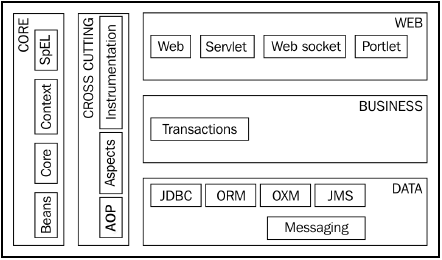
\includegraphics[scale=0.6]{img/019.png}
		\caption{Moduli di Spring}
		\label{fig: 019}
	\end{center}
\end{figure}
La modularità di Spring è uno dei suoi aspetti più importanti. La figura \ref{fig: 019} mostra i vari moduli, organizzati in base al loro layer di applicazione.
I principali aspetti di Spring sono:
\begin{itemize}
	\item IoC: non creare oggetti, delegalo al framework
	\item Dependency injection: 
	\item 
	\item 
	\item 
	\item 
\end{itemize}
\paragraph{Spring Core Container}
Fornisce la feature al centro di Spring, la dependency injection, tramite il container IOC (inversion of control)(paragrafo \ref{par: IOC}). I moduli del core di spring più importanti sono:
\begin{figure}[h!]
	\begin{center}
		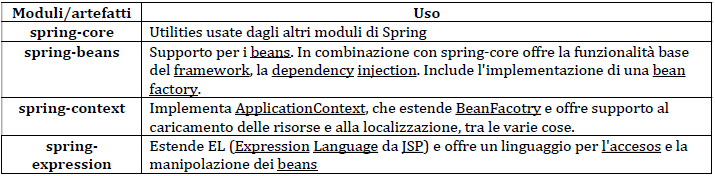
\includegraphics[scale=0.6]{img/020.png}
		\caption{Spring core}
		\label{fig: 020}
	\end{center}
\end{figure}
\paragraph{Problemi trasversali}
Certi problemi sono applicabili a tutti i livelli: log in, sicurezza, ecc. AOP è solitamente utilizzato per questi problemi.
\begin{figure}[h!]
	\begin{center}
		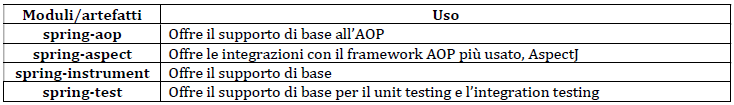
\includegraphics[scale=0.6]{img/021.png}
		\caption{Moduli per i problemi trasversali}
		\label{fig: 021}
	\end{center}
\end{figure}
\paragraph{Web}
Spring offre il suo framework MVC, Spring MVC. Due dei moduli più importanti sono:
\begin{itemize}
	\item spring-web
	\item spring-webmvc
\end{itemize}
\paragraph{Business}
Il livello di business si concentra sull'eseguire le operazioni logiche dell'applicazione. Solitamente vengono implementate tramite dei POJO (Plain Old Java Object). Le transazioni di Spring (spring-tx) offrono una gestione transazionale dichiarativa per queste classi.
\paragraph{Data}
Solitamente il livello dati para al database e alle interfacce esterne.
\begin{figure}[h!]
	\begin{center}
		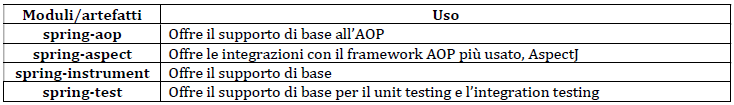
\includegraphics[scale=0.6]{img/021.png}
		\caption{Moduli per i dati}
		\label{fig: 022}
	\end{center}
\end{figure}

\section{Capitolo 2:Dependency injection}\label{par: IOC}
\footnote{Non c'è il capitolo 1 poichè era solo di introduzione}
Spring si occupa di creare e collegare gli oggetti grazie all'IoC container. 
Spring può "iniettare" dipendenze: immaginiamo di avere Interfaccia1, implementatta da B1, B2. Se A crea una new su Interfaccia1, spring la implementerà come B1 o B2 in base a ciò che serve.
\subsection{Comprendere la dependency injection}
Ora, immaginiamo di dover integrare all'interno di un servizio di business che richiede un qualche tipo di ordinamento, ad esempio bubble sort. Abbiamo due opzioni:
\begin{enumerate}
	\item Inserire all'interno della classe il codice dell'algoritmo
	\item Inserirlo in un'interfaccia, collegarla alla classe e successivamente collegarlo.
\end{enumerate}
Nel primo caso, in caso di cambiamenti all'algoritmo, avremo bisogno di modificare il codice per ogni classe che lo implementa, nel secondo caso dovremo modificarlo una sola volta.

A questo punto potremmo anche non far creare a BusinessServiceImpl un'istanza di DataServiceImpl, potremmo invece istanziarlo da un'altra parte per poi darlo a BusinessServiceImpl. Dobbiamo impostare quindi un setter per DataService
\begin{lstlisting}[language = Java]
public class BusinessServiceImpl {
	private DataService dataService;
	
	public void setDataService(DataService dataService) {
		this.dataService = dataService;
	}
	
	public long calculateSum(User user) {
		long sum = 0;
		for (Data data : dataService.retrieveData(user)) {
			sum += data.getValue();
		}
		return sum;
	}
}
\end{lstlisting}
Ora BusinessServiceImpl può lavorare con qualsiasi implementazione di DataService.

Ora, chi decide che istanza creare per DataServiceImpl? Ci pensa l'IOC container.

\subsection{IOC container}
3 domande compaiono:
\begin{enumerate}
	\item Come fa l'IOC container a sapere quale bean creare per le istanze?
	\item Come sa come collegare i bean assieme, ovvero come sa di dover "iniettare" l'istanza di DataserviceImpl in BusinessServiceImpl?
	\item Come sa dove cercare i bean?
\end{enumerate}

\subsubsection{Definire i bean e wiring}
Iniziamo con la prima domanda: 
\begin{center}
	\emph{"Come fa l'IOC container a sapere quale bean creare per le istanze?"}
\end{center}

Dobbiamo dire all'IOC container che bean creare. Possiamo farlo tramite le annotazioni $@$Repository, $@$Component, $@$Service sulle classi per le quali i bean devono essere creati. Queste annotazioni indicano a Spring di creare i bean per le classi specificate.

\textbf{$@$Component} è la maniera più generica per definire un bean. Le altre devono essere più specifiche per il contesto nel quale vengono usate. \textbf{$@$Service} è usata nei componenti di business, \textbf{$@$Repository} nei DAO.

Usiamo l'annotazione $@$Repository in DataServiceImpl perchè è legata all'accesso dati da un database (DAO). Usiamo $@$Service su BusinessServiceImpl perchè è un servizio di business.
\begin{lstlisting}[language = Java]
@Repository
public class DataServiceImpl implements DataService

@Service
public class BusinessServiceImpl implements BusinessService
\end{lstlisting}

Ora, prendiamo la seconda domanda: 
\begin{center}
	\emph{"Come sa come collegare i bean assieme, ovvero come sa di dover "iniettare" l'istanza di DataserviceImpl in BusinessServiceImpl?"}
\end{center}
Il bean di DataServiceImpl deve essere iniettato all'interno di BusinessServiceImpl. Possiamo farlo tramite l'annotazione \textbf{$@$Autowired} sulla variabile DataService nella classe BusinessServiceImpl.
\begin{lstlisting}[language = Java]
public class BusinessServiceImpl {
@Autowired
private DataService dataService;
\end{lstlisting}

\subsubsection{Creare un IOC container}
Ci sono due tipi di container IOC:
\begin{itemize}
	\item Bean factory: si occupa di tutte le funzionalità di base: il ciclo di vita dei bean e il loro wiring
	\item Application context: è un superset della bean factory con le funzionalità aggiuntive solitamente necessitate in un contesto enterprise. Viene consigliato di usare sempre questo a meno che non si lavori in un contesto dove l'ottimizzazione della memoria occupata non sia critica.
\end{itemize}

Per l'application contest possiamo usare una configurazione Java o una configurazione XML. Iniziamo con quella Java.

\paragraph{Configurazione Java per l'application context}
\begin{lstlisting}[language = Java]
@Configuration
class SpringContext {...}
\end{lstlisting}
Questo è un semplice esempio su come creare una configurazione di contesto Java. La chiave è l'annotazione \textbf{$@$Configuration}. \\
Rimane sempre la domanda "Come fa l'IOC container a sapere dove cercare i beans?".

Dobbiamo dire al container il package da cercare definendo una ricerca per le componenti. Aggiungiamo una nuova annotazione, \textbf{$@$ComponentScan}.
\begin{lstlisting}[language = Java]
@Configuration
@ComponentScan(basePackages = { "com.mastering.spring" })
class SpringContext {...}
\end{lstlisting}
Abbiamo ora definito la ricerca delle componenti all'interno del package com.mastering.spring.

Con ciò che abbiamo scritto fino ad ora, quando viene lanciato il contesto Spring:
\begin{itemize}
	\item Viene cercato com.mastering.spring e vengono trovati al suo interno BusinessServiceImpl e DataServiceImpl
	\item DataServiceImpl non ha dipendenze, viene quindi creato il bean
	\item BusinessServiceImpl ha dipendenze su DataService. DataServiceImpl è un'implementazione dell'interfaccia DataService, fa quindi matching sul criterio AutoWired. Quindi un bean BusinessServiceImpl viene creato e il bean creato per DataServiceImpl è AutoWired attraverso il setter..
\end{itemize}
\subparagraph{Lanciare l'application context con la configurazione Java}
\begin{lstlisting}[language = Java]
public class LaunchJavaContext {
	private static final User DUMMY_USER = new User("dummy");
	public static Logger logger =
		Logger.getLogger(LaunchJavaContext.class);
	
	public static void main(String[] args) {
		ApplicationContext context = 
			new AnnotationConfigApplicationContext(
			SpringContext.class);
			
		BusinessService service =
			context.getBean(BusinessService.class);
		logger.debug(service.calculateSum(DUMMY_USER));
	}
}
\end{lstlisting}
"ApplicationContext context =  new AnnotationConfigApplicationContext(SpringContext.class);" si occupa di creare l'application context. Una votla che il context è partito, dobbiamo ricevere il bean del BusinessService. Usiamo il metodo getBean che passa il tipo di bean come argomento (BusinessService.class):
\begin{lstlisting}[language = Java]
BusinessService service
	= 
context.getBean(BusinessService.class );
\end{lstlisting}

\paragraph{Configurazione XML per l'application context}
\subparagraph{Definire la configurazione Spring con XML}
Semplicemente si crea un file XML, in questo caso chiamato BusinessApplicationContext.xml, e si inserisce \textbf{"context: component-scan"}.
\begin{lstlisting}[language = XML]
<?xml version="1.0" encoding="UTF-8" standalone="no"?>
<beans> <!-Namespace definitions removed-->
	<context:component-scan base-package =
		"com.mastering.spring"/>
</beans>
\end{lstlisting}
\subparagraph{Lanciare l'application context con la configurazione XML}
\begin{lstlisting}[language = XML]
public class LaunchXmlContext {
	private static final User DUMMY_USER = 
		new User("dummy");
	public static Logger logger =
		Logger.getLogger(LaunchJavaContext.class);
	
	public static void main(String[] args) {
		ApplicationContext context = new
			ClassPathXmlApplicationContext(
			"BusinessApplicationContext.xml");
		BusinessService service =
			context.getBean(BusinessService.class);
		logger.debug(service.calculateSum(DUMMY_USER));
	}
}
\end{lstlisting}
"ApplicationContext context = new ClassPathXmlApplicationContext("BusinessApplicationContext.xml");" si occupa di creare l'application context.

\subsection{Tipi di dependency injection}
\paragraph{Setter injection}
Si usano i metodi setter. Ad esempio:
\begin{lstlisting}[language = Java]
public class BusinessServiceImpl {
	private DataService dataService;
	
	@Autowired
	public void setDataService
		(DataService dataService) {
		this.dataService = dataService;
	}
}

//_____________Altrimenti__________________

public class BusinessServiceImpl {
	@Autowired
	private DataService dataService;
}
\end{lstlisting}
Anche se, nella realtà, per usare una setter injection non serve nemmeno definire un metodo setter. Se si specifica $@$Autowired sulla variabile, Spring userà automaticamente la setter injection.
\paragraph{Costructor injection}
\begin{lstlisting}[language = Java]
public class BusinessServiceImpl {
	private DataService dataService;

	@Autowired
	public BusinessServiceImpl
		(DataService dataService) {
		super();
		this.dataService = dataService;
	}
}
\end{lstlisting}
Quando viene lanciato il codice si vedrà nel log una frase che spiega come l'autowiring sia avvenuto nel costruttore.
\paragraph{Setter vs constructor}
Solitamente la constructor injection veniva usata per le dipendenze obbligatorie, la setter per quelle facoltative. Bisogna però notare che quanto si usa @Autowired su di un campo o un metodo, la dipendenza è richiesta di default. Se non ci sono candidati all'autowire viene lanciata un'ipotesi. La scelta non è più così chiara quindi.

\subsection{Lo scope degli Spring beans}
I bean di spring pososno essere creati con multipli scope, singleton è quello di default. Lo scope può essere definito tramite l'annotazione \textbf{$@$Scope} su qualsiasi bean.
\begin{lstlisting}[language = Java]
@Service
@Scope("singleton")
public class BusinessServiceImpl implements BusinessService
\end{lstlisting}
\begin{figure}[h!]
	\begin{center}
		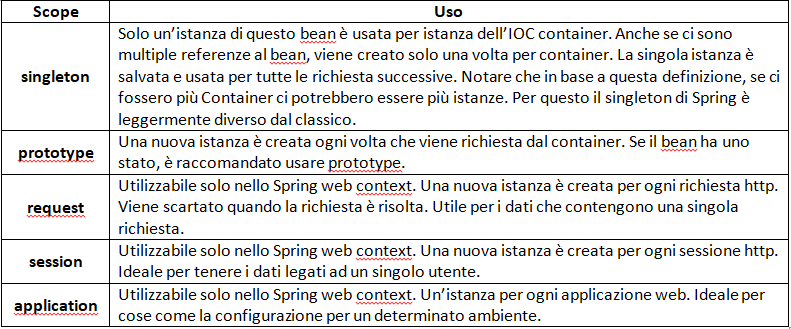
\includegraphics[scale=0.6]{img/023.png}
		\caption{Tipi di scope}
		\label{fig: 023}
	\end{center}
\end{figure}

\subsection{Annotazioni}
\begin{itemize}
	\item \textbf{$@$Controller}:
	\item \textbf{$@$RequestMapping}: cosa fare quando arriva un url. Deve esserci univocità di invocazione (url + metodo)
	\item \textbf{$@$ModelAttribute}: mettere sul model la variabile che si sta annotando e il nome sarà il nome della variabile
	\item \textbf{$@$Valid} (da hybernate): regola di validazione
	\item \textbf{$@$PathVariable}: associa il valore della variaible nell'url alla risorsa
	\item \textbf{$@$ResponseBody}: cosi facendo Spring scrive nel body la stringa restituita.
	\item \textbf{$@$AutoWired}: dependencies injection
	\item \textbf{$@$Primary}: quando è usata su di un bean, diventa il primo ad essere usato se ci sono più candidati.
	\item \textbf{$@$Qualifier}: serve ad indicare a Spring con quale bean specifico istanziare. Qua serve una spiegazione ulteriore\footnote{Vedi paragrafo \ref{par: qualifier}}
	\item \textbf{$@$PreDestroy}: Il metodo è chiamato prima che un bean venga rimosso dal container, rilascia tutte le risorse usate dal bean
\end{itemize}

Si inizia dal front controller (web.xml), tramite base package si vede dove cercare il controller d'ingresso, per sapere quando chiamare il controller si vede il mapping su cosa è eseguito.

\subsubsection{@Qualifier}\label{par: qualifier}
\begin{figure}[h!]
	\begin{center}
		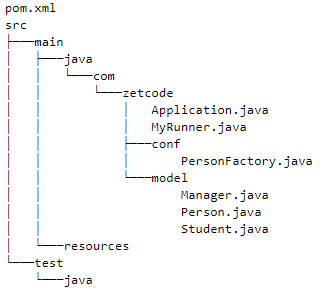
\includegraphics[scale=0.6]{img/024.png}
		\caption{Struttura classi}
		\label{fig: 024}
	\end{center}
\end{figure}
Qualifer serve a specificare a Spring quale classe istanziare. Bisogna associare ad ogni classe figlia il tag $@$Qualifier(Stringa di riconoscimento). Lo stesso tag verrà scritto sopra l'istanziazione per specificare il bean da usare.
\begin{lstlisting}[language = Java]
// Person.java
package com.zetcode.model;

public interface Person {

    String info();
}
//___________________________
// Student.java
package com.zetcode.model;

import org.springframework.beans.factory.annotation.Qualifier;
import org.springframework.stereotype.Component;

@Component
@Qualifier("student")
public class Student implements Person {

    @Override
    public String info() {

        return "Student";
    }
}
//___________________________
// Manager.java
package com.zetcode.model;

import org.springframework.beans.factory.annotation.Qualifier;
import org.springframework.stereotype.Component;

@Component
@Qualifier("manager")
public class Manager implements Person {

    @Override
    public String info() {
        return "Manager";
    }
}
//___________________________
// myRunner.java
@Component
public class MyRunner implements CommandLineRunner {

    private static final Logger logger = LoggerFactory.getLogger(MyRunner.class);

    @Autowired
    @Qualifier("student")// Speicifico che p1 e' uno studente
    private Person p1;

    @Autowired
    @Qualifier("manager") // Specifico che p2 e' un manager
    private Person p2;

    @Override
    public void run(String... args) throws Exception {

        logger.info("{}", p1.info());
        logger.info("{}", p2.info());
    }
}

\end{lstlisting}

\subsubsection{@Autowired} \label{par: Autowired}
Autowired può essere usato su proprietà, setter e costruttori.

\paragraph{Autowired e proprietà}
\begin{lstlisting}[language = Java]
@Component("fooFormatter")
public class FooFormatter {
 
    public String format() {
        return "foo";
    }
}
// _______________________________

@Component
public class FooService {
     
    @Autowired
    private FooFormatter fooFormatter;
 
}
\end{lstlisting}

Quando FooService viene creato, Spring genera automaticamente un FooFormatter e lo lega alla sua variabile

\subsubsection{Autowired e setter}
\begin{lstlisting}[language = Java]
public class FooService {
 
    private FooFormatter fooFormatter;
 
    @Autowired
    public void setFooFormatter(FooFormatter fooFormatter) {
            this.fooFormatter = fooFormatter;
    }
}
\end{lstlisting}
Quando FooService è creato viene automaticamente chiamato il metodo setFooFormatter con l'istanza di FooFormatter.

\subsubsection{Autowired e costruttori}
\begin{lstlisting}[language = Java]
public class FooService {
 
    private FooFormatter fooFormatter;
 
    @Autowired
    public FooService(FooFormatter fooFormatter) {
        this.fooFormatter = fooFormatter;
    }
}
\end{lstlisting}
QUando FooService viene ceato, un'istanza di FooFormatter è creata e usata come argomento del costruttore.

\subsubsection{@Primary}
Quando l'annotazione è utilizzata su di un bean, dievnta il primo ad essere usato nel caso ci siano più candidati.

\subsubsection{Annotazioni per la classe}
\paragraph{@Component}
È l'annotazione più generica per definire un bean

\paragraph{@Service}
Usato per definire le classi del service layer
\paragraph{@Repository}
Usato per definire i DAO
\paragraph{@Controller}
Usato per definire i controller\footnote{GAC}

\subsubsection{@Resource}
Mette assieme Autowired e Qualifier in una sola annotazione con sintassi @Resource(value="[qualifier]").

\subsubsection{@PostConstruct}
Usato su di un metodo di un bean. Il metodo viene chiamato una volta che il bean è inizializzato con le sue dipendenze. Viene chiamato una sola volta durante il ciclo di vita del bean.

\subsubsection{@PreDestroy}
Usato su di un metodo di un bean. Il metodo viene chiamato prima che il bean venga rimosso dal container. Può essere usato per rilasciare tutte le risorse trattenute dal bean.

\section{Capitolo 3: Creare un'applicazione web con Spring MVC}
Il modello è quello MVC con front controller.
\begin{figure}[h!]
	\begin{center}
		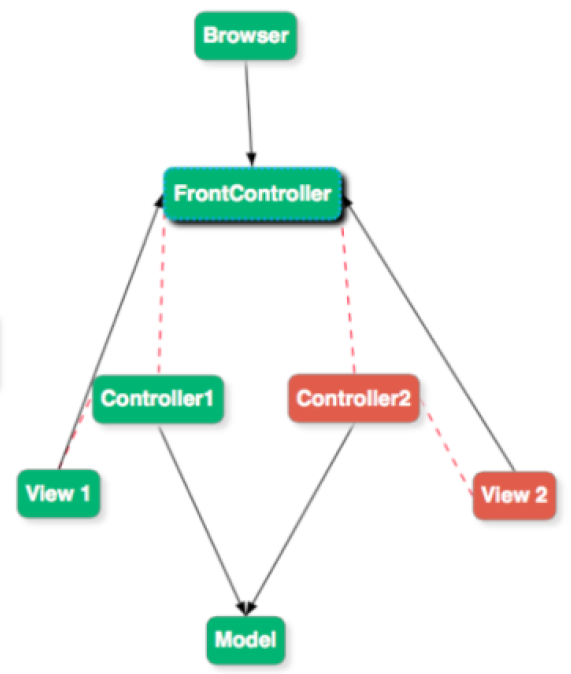
\includegraphics[scale=0.6]{img/025.png}
		\caption{MVC con front controller}
		\label{fig: 025}
	\end{center}
\end{figure}
In questo modello, i vari controller vengono chiamati da un controller primario che indirizza le richiste in base al contesto. Non vogliamo appesantire i controller con troppe funzioni, per questo c'è il front controller che contatterà i servizi necessari.
Alcune responsabilità di un tipico front controller:
\begin{enumerate}
	\item Decide quale controller esegue la richista
	\item decide quale view mostrare
	\item aggiunge funzionalità
	\item il front controller di Spring si chiama \textbf{DispatcherServlet}
\end{enumerate}

\subsection{Flow tipico}
Vedremo ora 6 tipici flow:
\begin{enumerate}
	\item Controller senza view: offre direttamente i contenuti (paragrafo \ref{flow1})
	\item Controller con view (JSP) (paragrafo \ref{flow2})
	\item Controller con view e con ModelMap (paragrafo \ref{flow3})
	\item Controller con view e con ModelAndView (paragrafo \ref{flow4})
	\item Controller per un semplice form (paragrafo \ref{flow5})
	\item Controller per un semplice form con validazione (paragrafo \ref{flow6})
\end{enumerate}

\subsubsection{Setup}
Prima di tutto dobbiamo impostare l'applicazione per l'uso di Spring MVC. Dobbiamo:
\begin{itemize}
	\item Aggiungere le dipendenze per SPring MVC
	\item Aggiungere DispatcherServlet a web.xml
	\item Creare un application context
\end{itemize}
\paragraph{Aggiungere le dipendenze per Spring MVC}
Iniziamo aggiungendo le dipendenze a pom.xml.
\begin{lstlisting}[language = XML]
<dependency>
	<groupId>org.springframework</groupId>
	<artifactId>spring-webmvc</artifactId>
</dependency>
\end{lstlisting}

\subsubsection{Aggiungere DispatcherServlet a web.xml}
Successivamente dobbiamo aggiungere il DispatcherServlet.
\begin{lstlisting}[language = XML]
<servlet>
	<servlet-name>
		spring-mvc-dispatcher-servlet
	</servlet-name>
	<servlet-class>
		org.springframework.web.servlet.DispatcherServlet
	</servlet-class>
	<init-param>
		<param-name>contextConfigLocation</param-name>
		<param-value>
			/WEB-INF/user-web-context.xml
		</param-value>
	</init-param>
	<load-on-startup>1</load-on-startup>
</servlet>

<servlet-mapping>
	<servlet-name>
		spring-mvc-dispatcher-servlet
	</servlet-name>
	<url-pattern>/</url-pattern>
</servlet-mapping>
\end{lstlisting}
La prima parte è per definire una servlet. Viene definita anche una cartella di configurazione, \emph{/WEB-INF/user-web-context.xml}. Nella seconda parte stiamo definendo un mapping, ovvero stiamo dicendo che questo controller gestirà tutte le pagine che iniziano con / (\emph{<url-pattern>/</url-pattern>}), quindi tutte.

\subsubsection{Creare un application context}
\begin{lstlisting}[language = XML]
<beans > <!-Schema Definition removed -->
	<context:component-scan
	base-package="com.mastering.spring.springmvc" />
	<mvc:annotation-driven />
</beans>
\end{lstlisting}
Con questo definiamo che la ricerca delle componenti sarà all'interno di com.mastering.spring.springmvc, in questo modo tutti i controller e i bean saranno creati e wired.

Usando l'annotazione \emph{<mvc:annotation-driven />} avviamo il supporto per una serie di feature come:
\begin{itemize}
	\item Mapping
	\item Gestione delle eccezioni
	\item Data binding e validazione
	\item Conversione automatica quando viene usata l'annotazione $@$RequestBody
\end{itemize}

\subsubsection{Flow 1 - Controller senza view} \label{flow1}
Iniziamo con un controller semplice:
\begin{lstlisting}[language = Java]
@Controller
public class BasicController {
	@RequestMapping(value = "/welcome")
	@ResponseBody
	public String welcome() {
		return "Welcome to Spring MVC";
	}
}
\end{lstlisting}
Parole chiave:
\begin{itemize}
	\item \textbf{$@$Controller}: definisce un controller che può contenere dei $@$RequestMapping
	\item \textbf{$@$RequestMapping(value = "/welcome")}: Definisce un mapping dell'URL legato al metodo welcome. Quando nel broser si accede alla sottopagina /welcome, Spring MVC esegue il metodo.
	\item \textbf{$@$ResponseBody}: In questo caso specifico, l'output del metodo viene mandato al browser come contenuto della risposta. La funzione di ResponseBody non si limita a questo però
\end{itemize}

\subsubsection{Flow 2 - Controller con view (JSP)} \label{flow2}
Nell'esempio precedente il testo da mostrare sul browser era all'interno del controller, pessima scelta dal punto di vista delle good practice. Generalemten il contenuto delle pagine è generato tramite View. Solitamente vengono usate le JSP, Java Server Pages.

\begin{lstlisting}[language = Java]
@Controller
public class BasicViewController {
	@RequestMapping(value = "/welcome-view")
	public String welcome() {
		return "welcome";
	}
}
\end{lstlisting}
\subsubsection{Flow 3 - Controller con view e con ModelMap} \label{flow3}
Generalmente per generare una view dovremmo passarle dei dati. In Spring possiamo passarle i dati usando un modello.
\begin{lstlisting}[language = Java]
@Controller
public class BasicModelMapController {
	@RequestMapping(value = "/welcome-model-map")
	public String welcome(ModelMap model) {
		model.put("name", "XYZ");
		return "welcome-model-map";
	}
}
\end{lstlisting}
Parole chiave:
\begin{itemize}
	\item $@$RequestMapping(value = "/welcome-model-map"): l'URI è mappata su /welcome-model-map
	\item public String welcome(ModelMap model:Il nuovo parametro agguinto + ModelMap model. Spring creerà un modello e lo renderà disponibile per quesot metodo. Gli attributi del modello saranno utilizzabili nella view
	\item model.put("name", "XYZ"): Aggiunge al modello un campo "name" con valore "XYZ"
\end{itemize}

Ora, per creare una vie creiamo una JSP in WEB-INF/views/welcome-model-map.jsp
\begin{lstlisting}[language = ]
Welcome ${name}! This is coming from a model-map - a JSP
\end{lstlisting}
\${name} usa la sintassi EL (Expression Language) per accedere all'attributo del modello.

\subsubsection{Flow 4 - Controller con view e con ModelAndView} \label{flow4}
Spring offre un approccio differente utilizzando ModelAndView. Il controller può ritornare un oggetto ModelAndView con il nome della view e gli appropriati attributi nel Model.
\begin{lstlisting}[language = Java]
@ControllerJava
public class BasicModelViewController {
	@RequestMapping(value = "/welcome-model-view")
	public ModelAndView welcome(ModelMap model) {
		model.put("name", "XYZ");
		return new ModelAndView("welcome-model-view", model);
	}
}
\end{lstlisting}
Parole chiave:
\begin{itemize}
	\item $@$RequestMapping(value = "/welcome-model-view"): l'URI è mappata su /welcome-model-view
	\item public ModelAndView welcome(ModelMap model): notare che il return non è una stringa ma una ModelAnd View
	\item return new ModelAndView("welcome-model-view", model): crae un oggetto ModelAndView con le appropriate view e modello.
\end{itemize}

Ora creiamo la view:
\begin{lstlisting}[language = ]
Welcome ${name}! This is coming from a model-view - a JSP
\end{lstlisting}
\subsubsection{Flow 5 - Controller per un semplice form} \label{flow5}
Ora concentriamoci sulla creazione di un semplice form per ricevere un input dall'utente. Si richiede:
\begin{itemize}
	\item Creare un semplice POJO, il bean dell'utente
	\item Creare una coppia di controller: uno per mostare il form e uno per catturare i dettagli inseriti in esso
	\item Creare una semplice view
\end{itemize}
I POJO sono generalmente usati per rappresentare i bean seguendo la tipica notazione JavaBean. Contengono le variabili private con i metodi getter e setter e il costruttore senza argomenti.
\begin{lstlisting}[language = Java]
public class User {
	private String guid;
	private String name;
	private String userId;
	private String password;
	private String password2;

	//Constructor
	//Getters and Setters
	//toString
}
\end{lstlisting}
Alcune cose importanti:
\begin{itemize}
	\item Questa classe non ha annotazioni di Spring
	\item Cattureremo nome, UserId e password nel form. abbiamo un campo di conferma password, pawwrod2, e un identificatore unico guid
	\item Costruttori, getter e setter e toString non sono mostrati solo per brevità
\end{itemize}

Controller:
\begin{lstlisting}[language = java]
@Controller
public class UserController {
	private Log logger = LogFactory.getLog
		(UserController.class);
		
	@RequestMapping(value = "/create-user",	method = RequestMethod.GET)
	public String showCreateUserPage(ModelMap model) {
		model.addAttribute("user", new User());
		return "user";
	}
}
\end{lstlisting}
Punti chiave:
\begin{itemize}
	\item $@$RequestMapping(value = "/create-user", method = RequestMethod.GET): stiamo mappando l'URI su /create-user. Per la prima volta abbiamo specificato una \emph{request} usando l'attributo method. QUesto metodo verrà invocato solo per le richieste HTTP GET. Non verrà invocato per altre azioni, tipo POST.
	\item public String showCreateUserPage(ModelMap model): tipico metodo di controllo
	\item model.addAtribute("user", new User()): per creare il modello con un bean vuoto dietro
\end{itemize}
Ora, le Java Server Pages (JSP)sono una delle tecnologie di Spring per supportare le view. Spring rede più semplice la creazione di views offrendo una libreria di tag. Qusti includono i tag per vari elementi dei form, binding, validazione, setting e messaggi multilingua.

Ora creiamo il file /WEB-INF/views/user.jsp.
Prima di tutto creiamo le reference alle librerie da usare:
\begin{lstlisting}[language = java]
<%@ taglib uri="http://java.sun.com/jsp/jstl/core" prefix="c"%>
<%@ taglib uri="http://java.sun.com/jsp/jstl/fmt" prefix="fmt"%>
<%@ taglib uri="http://www.springframework.org/tags/form" prefix="form"%>
<%@ taglib uri="http://www.springframework.org/tags" prefix="spring"%>
\end{lstlisting}
Le prime due entry sono per JSTL e per formattare le librerie di tag. Usiamo un prefisso (\emph{prefix}) per agire da scorciatoia per l'uso dei tag.
Ora creiamo il form:
\begin{lstlisting}[language = HTML]
<form:form method="post" modelAttribute="user">
	<fieldset>
		<form:label path="name">Name</form:label>
		<form:input path="name"
			type="text" required="required" />
	</fieldset>
</form:form>
\end{lstlisting}
Parole chiave:
\begin{itemize}
	\item <form:form method="post" modelAttribute="user">: Il tag form della libreria Spring con due attributi specificati: il metodo di invio (POST)  e il tipo di modello per la modellazione degli attributi dell'oggetto (user).
	\item <fieldset>: elemento HML per raggruppare una serie di controlli
	\item <form:label path="name">Name</form:label>: tag Spring per mostrare un'etichetta. Il apth specifica il nome del campo del bean al quale viene applicata questa etichetta
	\item <form:input path="name" type="text" required="required" />: Questo è il tag di Spring per creare un campo di input di testo. Il path specifica il campo del nome nel bean sul quale è mappato.
\end{itemize}
Quando usiamo il tag "form" di Spring, l'oggetto di backup (modelAttribute = "user) è collegato direttamente al form e inviando il form i valori vengono passati direttamente all'oggetto.

Per fare un esempio più completo:
\begin{lstlisting}[language = Java]
<form:form method="post" modelAttribute="user">
<form:hidden path="guid" />
<fieldset>
	<form:label path="name">Name</form:label>
	<form:input path="name"
		type="text" required="required" />
</fieldset>
<fieldset>
	<form:label path="userId">User Id</form:label>
	<form:input path="userId"
		type="text" required="required" />
</fieldset>
<!-password and password2 fields not shown for brewity-->
<input class="btn btn-success" type="submit" value="Submit" />
</form:form>
\end{lstlisting}

Quando l'utente fa il submit, il browser invoca una richiesta HTTP POST. Ora vedremo come creare un metodo per gestirla. Per rendere le cose semplici faremo anche un log dell'oggetto per mostrarlo direttamente.
\begin{lstlisting}[language = Java]
@RequestMapping(value = "/create-user", method = RequestMethod.POST)
public String addTodo(User user) {
	logger.info("user details " + user);
	return "redirect:list-users";
}
\end{lstlisting}
Parole chiave:
\begin{itemize}
	\item @RequestMapping(value = "/create-user", method = RequestMethod.POST): Poichè vogliamo gestire il submit del form usiamo il metodo RequestMethod.POST, così come indicato nel form
	\item public String addTodo(User user): Usiamo l'oggetto di backing del form come parametro. Spring MVC saprà automaticamente collegare i campi
	\item logger.info("user details " + user): viene loggato tutto
	\item return redirect:list-users: solitamente, una volta aggiornato il database, si reindirizza l'utente ad un'altra pagina. in questo caso a /list-user. QUando usiamo redirect Spring invia una HTTP response con status 302 che segnala un redirect ad una nuova URL
\end{itemize}

Il codice per mostrare tutti gli utenti è molto semplice:
\begin{lstlisting}[language = Java]
@RequestMapping(value = "/list-users", method = RequestMethod.GET)
public String showAllUsers() {
	return "list-users";
}
\end{lstlisting}

\subsubsection{Flow 6 - Controller per un semplice form con validazione} \label{flow6}
Nel precedente form non validavamo i valori. Mentre possiamo scrivere del codice Javascript per validarli (e per farci del male), è sempre meglio validare i dati a livello server.

Spring offre un'ottima implementazione con Bean Validation API, gestita tramite l'Hibernate validator.

Iniziamo aggiungendo il validatore al pom.xml:
\begin{lstlisting}[language = XML]
<dependency>
	<groupId>org.hibernate</groupId>
	<artifactId>hibernate-validator</artifactId>
	<version>5.0.2.Final</version>
</dependency>
\end{lstlisting}

E ora la magia, per semplicemente validare i campi basta aggiungere agli attributi del bean le annotazioni collegate:
\begin{lstlisting}[language = Java]
@Size(min = 6, 
	message = "Enter at least 6 characters")
private String name;

@Size(min = 6, 
	message = "Enter at least 6 characters")
private String userId;

@Size(min = 8, 
	message = "Enter at least 8 characters")
private String password;

@Size(min = 8, 
	message = "Enter at least 8 characters")
private String password2;
\end{lstlisting}
"message" è ciò che viene mostrato se la validazione non avviene.
Altre annotazioni per la validazione sono:
\begin{itemize}
	\item \textbf{@NotNull}: It should not be null
	\item \textbf{@Size(min =5, max = 50)}: Maximum size of 50 characters and minimum of 5 characters.
	\item \textbf{@Past}: Should be a date in the past
	\item \textbf{@Future}: Should be a future date
	\item \textbf{@Pattern}: Should match the provided regular expression
	\item \textbf{@Max}: Maximum value for the field
	\item \textbf{@Min}: Minimum value for the field
\end{itemize}
Vedere la lista completa nella \href{https://docs.jboss.org/hibernate/stable/validator/reference/en-US/html_single/#section-builtin-constraints}{documentazione di jboss}.

Ora, per scrivere nel controller di validare i campi, scriviamo:
\begin{lstlisting}[language = ]
@RequestMapping(value = "/create-user-with-validation",	method = RequestMethod.POST)
public String addTodo(@Valid User user, BindingResult result) {
	if (result.hasErrors()) {
		return "user";
	}
	logger.info("user details " + user);
	return "redirect:list-users";
}
\end{lstlisting}
Punti chiave:
\begin{itemize}
	\item public String addTodo($@$Valid User user, BindingResult result): QUando l'annotazione $@$Valid è usata, SPring valida il bean. Il risultato è reso disponibile tramite il BindingResult
	\item if (result.hasErrors()): Controlla se ci sono errori di validazione
	\item return "user": se ci sono errori di validazione l'utente viene rimandato alla pagina.
\end{itemize}

A questo punto dobbiamo potenziare la user.jsp per mostrare i messaggi di validazione. QUesto è un esempio, gli altri sono simili:
\begin{lstlisting}[language = Java]
<fieldset>
	<form:label path="name">Name</form:label>
	<form:input path="name" type="text" required="required" />
	<form:errors path="name" cssClass="text-warning"/>
</fieldset>
\end{lstlisting}

<form:errors path="name" cssClass="text-warning"/> è il tag di spring per mostrare gli errori relativi al campo nel path. Possiamo anche legare del CSS per mostrare meglio gli errori.

Se si vuole creare una validazione più complicata per motivi specifici si può usare l'annotazione \textbf{$@$AssertTrue}.
\begin{lstlisting}[language = ]
@AssertTrue(message = "Password fields don't match")
private boolean isValid() {
	return this.password.equals(this.password2);
}
\end{lstlisting}
$@$AssertTrue(message = "Password fields don't match") mostra il messaggio nel caso la validazione non sia effettuata.


\subsection{Come funziona Spring}
Nella sezione precedente abbiamo visto alcune delle feature più importanti:
\begin{itemize}
	\item Architettura a bassa dipendenza con ruoli indipendenti e ben definiti per ogni oggetto
	\item Controller altamente flessibile. I metodi del controller possono avere un vario range di parametri e valori di ritorno
	\item Permette il riuso degli oggetti come oggetti di backup collegati ai form frontend. Riduce il bisogno di avere form separati
	\item Tag built-in con supporto per la localizzazione
	\item Il modello usa una hashmap, permette un'integrazione con multiple tecnologie
	\item Binding flessibile. Gli errori durante la creazione possono essere gestiti come errori di validazione
	\item Mock MVC Framework per lo unit testing
\end{itemize}

\begin{figure}[h!]
	\begin{center}
		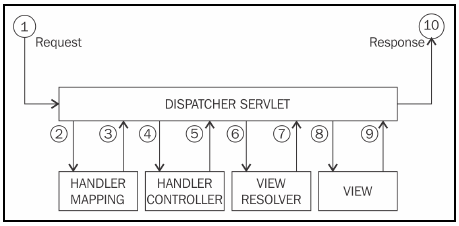
\includegraphics[scale=0.6]{img/032.png}
		\caption{Architettura Spring MVC}
		\label{fig: 032}
	\end{center}
\end{figure}
Ora prendiamo un flow di esempio e valutiamo i passi di esecuzione. Prendiamo il flow numero 4 (pagina \pageref{flow4}. L'URL è http://localhost:8080/welcome-model-view. Gli step sno:
\begin{enumerate}
	\item Il browser manda una richiesta per l'URL. La DispatcherServlet è il front controller e gestisce tutte le richieste. Riceve la richiesta
	\item La servlet controlla la URI (/welcome-model-view) e deve identificare i giusto controller per gestirla. Per trovare il controller giusto parla all'handler mapping
	\item L'handler mapping ritorna il metodo specifico (in questo esempio welcome in BasicModelViewController) che gestisce la richiesta
	\item La DispatcherServlet invoca il metodo specifico dell'handler (public ModelAndView welcome(ModelMap model)).
	\item Il metodo ritorna il modello e la view. In questo esempio un oggetto ModelAndView.
	\item DIsatcherServlet ha il nome logico della view (da ModelAndView \emph{welcome-model-view}). Ora deve capire come determinare il nome fisico della view. Controlla se ci sono dei view resolver disponibili. Trova il view resolver configurato (org.springframework.web.servlet.view.InternalResourceViewResolver). Chiama il resolver, dandogli il nome logico come input. 
	\item Il resolver esegue la logica per mappare il nome logico sul nome fisico. In questo caso welcome-model-view è tradotto in /WEB-INF/views/welcome-model-view.jsp
	\item Il DIspatcherServlet esegue la view. rende anche il modello disponibile alla view
	\item La view ritorna il contenuto per essere inviato alla DispatcherServlet
	\item La DispatcherServlet invia la risposta al browes
\end{enumerate}

Ora possiamo effettivamente capire alcuni concetti importanti di Spring.
\subsubsection{RequestMapping}
$@$RequestMapping è usato per mappare una URI ad un controller o ad un metodo del controller. Un parametro aggiuntivo, RequestMethod, permette di mappare il metodo ad una specifica richesta (POST, GET, ecc.)

Metodi accettati sugli argomenti dei metodi con RequestMapping:
\begin{itemize}
	\item java.util.Map / org.springframework.ui.Model / org.springframework.ui.ModelMap: agisce come modello che conterra i valori che sono esposti alla view
	\item oggetti form o comandi: usati per legare le richieste ai parametri dei bean. Supportano la validazione
	\item org.springframework.validation.Errors / org.springframework.validation.BindingResult: risultato della validazione
	\item $@$PreDestroy: su ogni bean, questo metodo è chiamato prima che un bean venga rimosso dal container. Può essere usato per rilasciare le risorse bloccate dal bean
	\item $@$RequestParam: L'annotazione per accedere ad un parametro HTTP specifico
	\item $@$RequestHeader: l'annotazione per accedere ad un header HTTP specifico
	\item $@$SessionAttribute: l'annotazione per accedere ad un attributo specifico della session
	\item $@$RequestAttribute: l'annotazione per accedere ad un attributo specifico della richiesta HTTP
	\item $@$PathVariabile: l'annotazione che permette l'accesso alle variabili dell'URI. Capiremo meglio coi microservizi
\end{itemize}

$@$RequestMapping supporta una varietà di tipi di ritorno. Pensando concettualmente, un metodo con RequestMapping dovrebbe rispondere a due domande:
\begin{enumerate}
	\item Qual è la view?
	\item Qual è il modello che la view necessita?
\end{enumerate}

Nonostante ciò, con Spring, view e model possono non essere dichiarati esplicitamente tutte le volte:
\begin{itemize}
	\item Se una view non è esplicitamente definita come tipo di ritorno, allora è definita implicitamente
	\item Similmente, qualsiasi oggetto è sempre arricchieto come descritto più sotto
\end{itemize}

Spring usa una semplice regola per determinare le esatte view e model. Una coppia di regole importanti:
\begin{itemize}
	\item \textbf{Arricchimento implicito del modello}: se un modello fa parte del tipo di ritorno, è arricchito con o dei comandi (inclusi i risultati dalle validazioni). In aggiunta, i risultati dei metodi con l'annotazione $@$ModelAttributte sono aggiunti al modello.
	\item \textbf{Implicita determinazione della view}: se il nome della view non è nel tipo di ritorno, è determinata usando DefaultRequestToViewNameTranslator. Di default rimuove lo slash di inizio e di fine così come l'estensione del file dall'URI (ad esempio display.html diventa display)
\end{itemize}
I tipi di ritorno che sono supportati sui metodi del Controller con RequestMapping:
\begin{itemize}
	\item \textbf{ModelAndView}: l'oggetto include un puntatore al modello e al nome della view
	\item \textbf{Model}: solo il modello viene ritornato, il nome della view è determinato tramite il  DefaultRequestToViewNameTranslator
	\item \textbf{Map}: Una semplice map è usata per esporre un modello
	\item \textbf{View}:una view con un modello implicitamente definito
	\item \textbf{String}: puntatore al nome della view
\end{itemize}

\subsubsection{View resolution}
Spring offre una view resolution flessibile. Offre varie opzioni:
\begin{itemize}
	\item Integrazione con JSP, freemaker
	\item Varie strategie di view resolution, alcune delle quali sono:
	\begin{itemize}
		\item \textbf{XmlViewResolver}: Basata su di un file esterno di configurazione XML
		\item \textbf{ResourceBundleViewResolver}: basata su di un file di proprietà
		\item \textbf{UrlBasedViewResolver}: mapping diretto del nome logico della view all'URL
		\item \textbf{ContentNegotiatingViewResolver}: delega ad altri resolver basato sull'header request Accept
	\end{itemize}
	\item Supporto per il cambio di view resolver con definizione esplicita dell'ordine di preferenza
	\item Generazione diretta di XML, JSON e Atom usando la content Negotiation
\end{itemize}

Un esempio di InternalResourceViewResolver è:
\begin{lstlisting}[language = XML]
<bean id="jspViewResolver" class=
	"org.springframework.web.servlet.view.
	InternalResourceViewResolver">
	<property name="viewClass"
		value="org.springframework.web.servlet.view.JstlView"/>
	<property name="prefix" value="/WEB-INF/jsp/"/>
	<property name="suffix" value=".jsp"/>
</bean>
\end{lstlisting}
Il nome fisico della view è determinato usando prefisso e suffisso determinati per la logical view usando JstlView.

\paragraph{Configurare Freemarker}
Prima di tutto configuriamo il bean usato per caricare i template di Freemarker.
\begin{lstlisting}[language = XML]
<bean id="freemarkerConfig"
	class="org.springframework.web.servlet.view.
	freemarker.FreeMarkerConfigurer">
	<property name="templateLoaderPath" value="/WEBINF/freemarker/"/>
</bean>
\end{lstlisting}

Ora ecco il bean per configurare il view resolver
\begin{lstlisting}[language = XML]
<bean id="freemarkerViewResolver"
	class="org.springframeowork.web.servlet.view.freemarker.FreeMarkerViewResolver">
	<property name="cache" value="true"/>
	<property name="prefix" value=""/>
	<property name="suffix" value".ftl"/>
</bean>
\end{lstlisting}

\subsubsection{Attributi dei Model}
Solitamente i form online contengono una lista di valori dai menù drop down (ad esempio una lista di stati, una lista di titoli ecc.). QUesta lista deve essere resa disponibile al Model e per farlo si usa l'annotazione @ModelAttribute legata ai metodi.
\begin{lstlisting}[language = Java]
@ModelAttribute
public List<State> populateStateList() {
	return stateService.findStates();
}

	// Per piu' attributi

@ModelAttribute
public void populateStateAndCountryList() {
	model.addAttribute(stateService.findStates());
	model.addAttribute(countryService.findCountries());
}
\end{lstlisting}

Non c'è una limitazione ai metodi che possono essere segnati tramite @ModelAttribute.

I Model attribute possono esseere resi accessibili tra più controller usando Controller Advice.

\subsubsection{Attributi della Session}
I successivi attributi vengono usati in una singola richiesta. Comunque ci potrebbero essere valori specifici dello user che non verranno condivisi tra le richiesta. Questi valori solitamente sono salvati nell'HTTP session. Spring MVC offre una semplice annotazione a livello di classe o di tipo, @SessionAttributes per specificare questi attributi:
\begin{lstlisting}[language = Java]
@Controller
@SessionAttributes("exampleSessionAttribute")
public class LoginController {
	...
	model.put("exampleSessionAttribute", sessionValue);
	...
}
\end{lstlisting}

Una volta che definiziamo un attributo nell'annotazione, è automaticamente aggiunto alla sessione se lo stesso attributo è aggiunto al Model. Se ad un certo punto nel controller aggiungiamo un attributo con lo stesso nome al model, questo verrà aggiunto anche alla sessione.

Il valore può essere reso accessibile in altri controller specirficando l'annotazione @SessionAttribute a livello di tipo. Il valore sarà reso automaticamente disponibile a tutti e potrà essere accessibile tramite model:
\begin{lstlisting}[language = Java]
@Controller
@SessionAttributes("exampleSessionAttribute")
public class SomeOtherController {
	...
	Value sessionValue = (Value)model.get("exampleSessionAttribute");
	...
}
\end{lstlisting}

È impostante rimuovere dalla sessione i valori che non sono più necessari. Ci sono due modi per rimuoverli:
\begin{enumerate}
	\item usare removeAttribute accessibile tramile la classe WebRequest
	\item usare il metodo cleanUpAttribute
\end{enumerate}
\begin{lstlisting}[language = Java]
// Metodo 1
@RequestMapping(value="/some-method", method = RequestMethod.GET)
public String someMethod(/*Other Parameters*/
	WebRequest request, SessionStatus status) {
	status.setComplete();
	request.removeAttribute("exampleSessionAttribute", WebRequest.SCOPE_SESSION);
	//Other Logic
}

// Metodo 2
@RequestMapping(value = "/some-other-method", method = RequestMethod.GET)
public String someOtherMethod(/*Other Parameters*/
	SessionAttributeStore store, SessionStatus status) {
	status.setComplete();
	store.cleanupAttribute(request, "exampleSessionAttribute");
	//Other Logic
}
\end{lstlisting}

La personalizzazione del binding viene effettuata tramite @InitBinder. La personalizzazione può essere fatta in uno specirfico controller o in più controller usando Handler Advice.
\begin{lstlisting}[language = Java]
@InitBinder
protected void initBinder(WebDataBinder binder) {
	SimpleDateFormat dateFormat = new SimpleDateFormat("dd/MM/yyyy");
	binder.registerCustomEditor(Date.class,	new CustomDateEditor(dateFormat, false));
}
\end{lstlisting}
Questo codice, ad esemio, impone come verrà configurata la data per tutte le sue occorrenze.

Fondamentalmente InitBinder funziona come un preprocessore dei dati inviati al controller.

\begin{lstlisting}[language = Java]
vinder.registerCustomEditor(
	[classe alla quale applicare il metodo], 
	[classe da associare per l'editing])
\end{lstlisting}

\subsection{Feature avanzate}
\subsubsection{Gestione delle eccezioni}
Con Spring la maggior parte delle eccezioni è resa unchecked. QUesto permette di gestirle in maniera generale.

Due metodi di gestione delle eccezioni sono:
\begin{enumerate}
	\item Gestione comune a tutti i controller
	\item Eccezioni specifiche per un contoller
\end{enumerate}

\paragraph{Gestione comune a tutti i controller}
Controller advice può essere usato anche per implementare una gestione comune delle eccezioni tra vari controller:
\begin{lstlisting}[language = Java]
@ControllerAdvice
public class ExceptionController {
	private Log logger = LogFactory.getLog(ExceptionController.class);
	
	@ExceptionHandler(value = Exception.class)
	public ModelAndView handleException	(HttpServletRequest request, Exception ex) {
		
		logger.error("Request " + request.getRequestURL() + " Threw an Exception", ex);
		ModelAndView mav = new ModelAndView();
		mav.addObject("exception", ex);
		mav.addObject("url", request.getRequestURL());
		mav.setViewName("common/spring-mvc-error");
		return mav;
	}
}
\end{lstlisting}
Notiamo alcune parti:
\begin{itemize}
	\item \textbf{@ControllerAdvice}: è applicabile a tutti i controller
	\item \textbf{@ExceptionHandler(value = Exception.class)}: ogni metodo con questa annotazione sarà chiamato quando un'eccezione di quel sottotitpo verrà lanciata
	\item \textbf{public ModelAndView handleException(HttpServletRequest request, Exception ex)}: l'eccezione che viene lanciata è injected nella variabile Exception. Il metodo è dichiarato con un tipo di ritorno ModelAndView per permettere al controller di restituire un model con l'eccezione gestita e una view di gestione.
	\item\textbf{ mav.addObject("exception", ex)}: aggiungere un'eccezione al model in modo che possa essere visualizzata nella view
	\item \textbf{mav.setViewName("common/spring-mvc-error")}: la view dell'eccezione
\end{itemize}

E la view di errore:
\begin{lstlisting}[language = HTML]
<%@ taglib prefix="c" uri="http://java.sun.com/jsp/jstl/core"%>
<%@page isErrorPage="true"%>
<h1>Error Page</h1>
URL: ${url}
<br />
Exception: ${exception.message}
<c:forEach items="${exception.stackTrace}"
	var="exceptionStackTrace">
	${exceptionStackTrace}
</c:forEach>
\end{lstlisting}

Notiamo che:
\begin{itemize}
	\item \textbf{URL: \$\{url\}}: mostra l'URL del model
	\item \textbf{Exception: \$\{exception.message\}}: mostra il messaggio dell'eccezione. L'eccezione è popolata nel model da ExceptionController
	\item \textbf{forEach around \$\{exceptionStackTrace\}}: mostra la stack trace
\end{itemize}

\paragraph{Gestione specifica in un Controller}
Si può lavorare nello stesso modo, semplicemente l'annotazione sarà posta a livello di metodo all'interno del controller.

\subsection{Internazionalizzazione (I18N)}
Può essere implementata usando due approcci:
\begin{itemize}
	\item SessionLocaleResolver
	\item CookieLocaleResolver
\end{itemize}
Nel primo caso, il locale scelto dallo user è salvato nella sessione e, quindi, viene mantenuto solo durante quella sessione. Nell'altro caso invece diventa comune a più sessioni.

\subsubsection{Message bundle setup}
Prima di tutto, prepariamo il message bundler. Lo snippet è questo:
\begin{lstlisting}[language = XML]
<bean id="messageSource" class=
	"org.springframework.context.support.ReloadableResourceBundleMessageSource">
	<property name="basename" value="classpath:messages" />
	<property name="defaultEncoding" value="UTF-8" />
</bean>
\end{lstlisting}
Notiamo:
\begin{itemize}
	\item \textbf{class="org.springframework.context.support.ReloadableResourceBu
ndleMessageSource"}: siamo configurando un reloadable resource bundle. Permette il ricaricamento delle proprietà trmaite cache
	\item \textbf{$<property name="basename" value="classpath:messages" />$}: configura il caricamento delle proprietà tramite messages.properties e il file messages\_{locale}.properties.
\end{itemize}
Configuriamo una coppia di file di proprietà e rendiamoli accessibili in src/main/resources:
\begin{lstlisting}[language =]
// message_en.properties
welcome.caption=Welcome in English

// message_fr.properties
welcome.caption=Bienvenue - Welcome in French
\end{lstlisting}
Possiamo mostrare i messaggi usando il tag spring:message:
\begin{lstlisting}[language = HTML]
<spring:message code="welcome.caption" />
\end{lstlisting}

\subsubsection{Configurare un SessionLocaleResolver}
Ci sono due parti del configurare un SessionLocaleResolver:
\begin{enumerate}
	\item configurare un localeResolver
	\item configurare un interceptor per gestire i cambiamenti del locale
\end{enumerate}

\begin{lstlisting}[language = XML]
<bean id="springMVCLocaleResolver"
	class="org.springframework.web.servlet.i18n.SessionLocaleResolver">
	<property name="defaultLocale" value="en" />
</bean>

<mvc:interceptors>
	<bean id="springMVCLocaleChangeInterceptor"
		class="org.springframework.web.servlet.i18n.LocaleChangeInterceptor">
		<property name="paramName" value="language" />
	</bean>
</mvc:interceptors>
\end{lstlisting}

Notiamo:
\begin{itemize}
	\item \textbf{<property name="defaultLocale" value="en" />}: di default il locale è en
	\item \textbf{<mvc:interceptors>}: LocaleChangeInterceptor è configurato come un HandlerInterceptor. Intercetta tutte le richieste agli handler e controlla il locale
	\item \textbf{<property name="paramName" value="language" />}: LocaleChangeInterpetor è configurato per usare un parametro dalla HTTP request chiamato language che indica il locale. Quindi qualsiasi URL nel formato \emph{http://server/uri?language={locale}} genererebbe un cambio del locale
	\item Se aggiungi language=en a qualsiasi URL, segnali di usare en per tutta la durata della sessione.
\end{itemize}

\subsubsection{Configurare un CookieLocaleResolver}
Usiamo un CookieLocaleResolver così:
\begin{lstlisting}[language = XML]
<bean id="localeResolver"
	class="org.springframework.web.servlet.i18n.CookieLocaleResolver">
	<property name="defaultLocale" value="en" />
	<property name="cookieName" value="userLocaleCookie"/>
	<property name="cookieMaxAge" value="7200"/>
</bean>
\end{lstlisting}
Notiamo:
\begin{itemize}
	\item \textbf{<property name="cookieName" value="userLocaleCookie"/>}: il nome del cookie salvato nel browser
	\item \textbf{<property name="cookieMaxAge" value="7200"/>}: la durata del cookie è di due ore (7200 secondi)
	\item  poichè stiamo usando un LocaleChangeInterceptor, se si aggiunge language=en a qualsiasi URL, si userebbe il locale en per due ore ( o fino a cambiamento)
\end{itemize}

\subsection{Integration testing dei controller}
Caricando l'intero context per controllare l'integrazione dei controller staremmo parlando di \textbf{Integration testing}.
\begin{lstlisting}[language = Java]
@RunWith(SpringRunner.class)
@WebAppConfiguration
@ContextConfiguration("file:src/main/webapp/WEB-INF/user-web-context.xml")
public class BasicControllerSpringConfigurationIT {
	
	private MockMvc mockMvc;

	@Autowired
	private WebApplicationContext wac;

	@Before
	public void setup() {
		this.mockMvc =
			MockMvcBuilders.webAppContextSetup
				(this.wac).build();
	}

	@Test
	public void basicTest() throws Exception {
		this.mockMvc
			.perform(get("/welcome")
				.accept(MediaType.parseMediaType("application/html;charset=UTF-8")))
			.andExpect(status().isOk())
			.andExpect(content().string("Welcome to Spring MVC"));
	}
}
\end{lstlisting}

Analizziamolo:
\begin{itemize}
	\item \textbf{@RunWith(SpringRunner.class)}: SpringRunner ci aiuta nel lanciare uno SpringContext
	\item \textbf{@WebAppConfiguration}: Usato per lanciare una web app con Spring MVC
	\item \textbf{@ContextConfiguration("file:src/main/webapp/WEB-INF/user-webcontext.
xml")}: specifica il path dell'XML con il contesto di Spring
	\item \textbf{this.mockMvc =
MockMvcBuilders.webAppContextSetup(this.wac).build()}: Nei primi esempi abbiamo usato un setup standalone. In questo esempio, invece, lanciamo l'intera web app, per questo usiamo webAppContextSetup
	\item  L'esecuzione è simile agli altri test
\end{itemize}

\subsection{Offrire risorse statiche}
Il backend, generalmente, viene costruito tramite applicazioni web o servizi REST basati su framework come Spring MVC.

Spring MVC offre alcune feature importanti:
\begin{itemize}
	\item espongono il contenuto statico dalle cartelle nel web application root
	\item abilita il caching
	\item abilita la compressione Gzip del contenuto statico
\end{itemize}

\paragraph{Esposizione del contenuto statico}
Le applicazioni web solitamente hanno molti contenuti statici. Spring MVC offre possibilità per esporre questi contenuti direttamente da cartelle specifiche. d esempio:
\begin{lstlisting}[language = HTML]
<mvc:resources
	mapping="/resources/**"
	location="/static-resources/"/>
\end{lstlisting}

Notare:
\begin{itemize}
	\item \textbf{location="/static-resources/"}: La location indica la cartella all'interno del file war o del classpath che vogliamo esporre come contenuto statico. In questo esempio è all'interno della cartella static-resources partendo dal root. Possiamo anche specificare più cartelle usando valori separati da virgole
	\item \textbf{mapping="/resources/**"}: il mapping specifica l'URI utilizzata per accedere al path. Quindi, ad esempio, un file CSS chiamato app.css all'interno della cartella statica sarebbe usato tramite /resources/app.css
\end{itemize}

La configurazione completa in Java è:
\begin{lstlisting}[language = Java]
@Configuration
@EnableWebMvc
public class WebConfig extends WebMvcConfigurerAdapter {
	
	@Override
	public void addResourceHandlers
		(ResourceHandlerRegistry registry) {
		registry
			.addResourceHandler("/static-resources/**")
			.addResourceLocations("/static-resources/");
	}
}
\end{lstlisting}

\subsubsection{Caching}
Viene effettuato sia a livello di classe che a livello di XML:
\begin{lstlisting}[language = Java]
// Classe
registry
	.addResourceHandler("/resources/**")
	.addResourceLocations("/static-resources/")
	.setCachePeriod(365 * 24 * 60 * 60);
\end{lstlisting}
\begin{lstlisting}[language = XML]
<!-- XML -->
<mvc:resources
	mapping="/resources/**"
	location="/static-resources/"
	cache-period="365 * 24 * 60 * 60"/>
\end{lstlisting}
L'header Cache-Control: max-age={specified-max-age} verrà mandato al browser.

\subsubsection{Abilitare la compressione GZip}
Comprimere una response in maniera semplice è un modo molto semplice per rendere un'applicazione web più veloce. Tutti i browser usano Gzip. La compressione e la decompressione sono trasparenti per il browser.

Semplicemente il browser può specificare se accetta contenuto compresso o no. Se il server lo supporta, può essere usato.

La request Header inviata dal browser è: \emph{Accept-Encoding: gzip, deflate}

La response header inviata dalla web application è: \emph{Content-Encoding: gzip}

Ad esempio:
\begin{lstlisting}[language = Java]
registry
	.addResourceHandler("/resources/**")
	.addResourceLocations("/static-resources/")
	.setCachePeriod(365 * 24 * 60 * 60)
	.resourceChain(true)
	.addResolver(new GzipResourceResolver())
	.addResolver(new PathResourceResolver());
\end{lstlisting}

Notiamo:
\begin{itemize}
	\item \textbf{resourceChain(true)}: Serve per controllare che sia effettivamente possibile inviare file compressi, altrimenti verrà inviato il file completo. Per questo usiamo la resource chain
	\item \textbf{addResolver(new PathResourceResolver())}:  PathResourceResolver è il resolver di base
	\item \textbf{addResolver(new GzipResourceResolver())}: abilita la compressione
\end{itemize}

\subsection{Integrare Spring MVC con Bootstrap}
WebJars ci permette di gestire le versioni di bootstrap tramite Maven. WebJars sono file jar lato client che contengono JS  CSS. Possiamo usare Maven o Gradle per scaricarli e renderli disponibili all'applicazione. Il vantaggio di WebJars è che risolve le dipendenze transitive.

I passi sono:
\begin{enumerate}
	\item aggiungere Bootstrap Webjar come dipendenza di Maven
	\item configurare l'MVC resource handler per usare il contenuto statico da WebJars
	\item Usare le risorse di Bootstrap nelle JSP
\end{enumerate}

\subsubsection{Aggiungere Bootstrap Webjar come dipendenza di Maven}
Semplicemente lo aggiungiamo al file pom.xml:
\begin{lstlisting}[language = XML]
<dependency>
	<groupId>org.webjars</groupId>
	<artifactId>bootstrap</artifactId>
	<version>x.y.z</version>
</dependency>
\end{lstlisting}

\subsubsection{Configurare l'MVC resource handler per usare il contenuto statico da WebJars}
Anche questo passaggio è molto semplice. Nello spring context aggiungiamo:
\begin{lstlisting}[language = XML]
<mvc:resources 
	mapping="/webjars/**" 
	location="/webjars/"/>
\end{lstlisting}

Con questa configurazione il ResourceHttpRequestHandler rende disponibile il contenuto del WebJars come contenuto statico.

\subsubsection{Usare le risorse di Bootstrap nelle JSP}
Possiamo usarle come ogni altro contenuto statico:
\begin{lstlisting}[language = HTML]
<script src=
	"webjars/bootstrap/3.3.6/js/bootstrap.min.js">
</script>
<link
	href="webjars/bootstrap/3.3.6/css/bootstrap.min.css"
	rel="stylesheet">
\end{lstlisting}

\subsection{Spring Security}
L'autenticazione è il processo di stabilire l'identità dello user, verificando che sia chi dice di essere.

L'autorizzazione è controllare che abbia i permessi per svolgere una determinata azione.

Una best practice è di rinforzare l'autenticazione e l'autorizzazione su ogni pagina.

Spring security supporta la maggior parte dei meccanismi di autenticazione:
\begin{itemize}
	\item Form-based
	\item LDAP
	\item JAAS
	\item basati sui container
	\item sistemi custom
\end{itemize} 

Proviamo a creare  una semplice applicazione con SPring Security. I passi sono:
\begin{enumerate}
	\item Aggiungere le dipendenza da Spring Security
	\item Configurare l'intercettazione di tutte le richieste
	\item Configurare Spring Security
	\item Aggiungere una funzionalità di logout
\end{enumerate}

\subsubsection{Aggiungere le dipendenza da Spring Security}
La dipendenza, come sempre, va aggiunta al file pom.xml:
\begin{lstlisting}[language = XML]
<dependency>
	<groupId>org.springframework.security</groupId>
	<artifactId>spring-security-web</artifactId>
</dependency>
<dependency>
	<groupId>org.springframework.security</groupId>
	<artifactId>spring-security-config</artifactId>
</dependency>
\end{lstlisting}

\subsubsection{Configurare l'intercettazione di tutte le richieste}
La best practice è quella di validare tutte le richieste HTTP. Bisogna farlo tramite un filtro che intercetti tutte le richieste e le convalidi. Useremo un filtro, DelegatingFilterProxy, che delega ad un bean di Spring FilterChainProxy:
\begin{lstlisting}[language = XML]
<filter>
	<filter-name>springSecurityFilterChain</filter-name>
	<filter-class>
		org.springframework.web.filter.DelegatingFilterProxy
	</filter-class>
</filter>

<filter-mapping>
	<filter-name>springSecurityFilterChain</filter-name>
	<url-pattern>/*</url-pattern>
</filter-mapping>
\end{lstlisting}

\subsubsection{Configurare Spring Security}
Usiamo, come sempre, un file di configurazione:
\begin{lstlisting}[language = Java]
@Configuration
@EnableWebSecurity
public class SecurityConfiguration extends WebSecurityConfigurerAdapter {
	
	@Autowired
	public void configureGlobalSecurity	(AuthenticationManagerBuilder auth) throws Exception {
		auth.inMemoryAuthentication()
			.withUser("firstuser")
			.password("password1")
			.roles("USER", "ADMIN");
	}

	@Override
	protected void configure(HttpSecurity http)	throws Exception {
		http.authorizeRequests()
			.antMatchers("/login")
			.permitAll()
			.antMatchers("/*secure*/**")
			.access("hasRole('USER')")
			.and().formLogin();
	}
}
\end{lstlisting}

Notiamo:
\begin{itemize}
	\item \textbf{@EnableWebSecurity}: L'annotazione consente ad ogni classe di configurazione di contenere la configurazione di Spring. In questo caso, facciamo l'override di un paio di metodi per offrire la nostra configurazione specifica.
	\item \textbf{WebSecurityConfigurerAdapter}: questa classe offre una classe base per creare un Confiurazione di Spring
	\item \textbf{protected void configure(HttpSecurity http)}: QUesto metodo offre la sicurezza richiesta per differenti URL
	\item \textbf{antMatchers("/*secure*/**").access("hasRole('USER')")}: serve un ruolo da USER per accedere a qualsiasi URL che contenga la sottostringa "secure"
	\item \textbf{antMatchers("/login").permitAll()}: Permette a tutti gli utenti di accedere alla pagina di login
	\item \textbf{public void configureGlobalSecurity(AuthenticationManagerBuilder auth)}: in questo esempio stiamo usando un autenticatore in memoria. Può essere usato per connettersi ad un database (auth.jdbcAuthentication()) o un LDAP (auth.ldapAuthentication()),  o un provider personalizzato
	\item \textbf{withUser("firstuser").password("password1")}: configura una combinazione User-PWD valido in memoria
	\item \textbf{.roles("USER", "ADMIN")}: Assegna un ruolo ad un utente
\end{itemize}

Quando proviamo ad accedere ad'URL sicura, saremo reindirizzati alla pagina di login. Spring Security offre maniere di personalizzare la logica della pagina così come il reindirizzamento. 

\subsubsection{Aggiungere una funzionalità di logout}
Spring Security offre soluzioni per permettere all'utente di fare il oog out ed essere reindirizzato verso pagine specifiche. L'URI del LogoutController solitamente è mappata sul link di logout della UI.
\begin{lstlisting}[language = Java]
@Controller
public class LogoutController {

	@RequestMapping(value = "/secure/logout", method = RequestMethod.GET)
	public String logout(HttpServletRequest request,
		HttpServletResponse response) {
	
		Authentication auth = SecurityContextHolder.getContext()
			.getAuthentication();
		if (auth != null) {
			new SecurityContextLogoutHandler()
				.logout(request, response, auth);
			request.getSession().invalidate();
		}
		
		return "redirect:/secure/welcome";
	}
}
\end{lstlisting}
	
Notare:
\begin{itemize}
	\item \textbf{if(auth != null)}: Controlla che l'autenticazione sia valida
	\item \textbf{new SecurityContextLogoutHandler().logout(request, response, auth)}: SecurityContextLogoutHandler esegue un logout rimuovendo le informazioni di autenticazione da SecurityContextHolder
	\item \textbf{return "redirect:/secure/welcome"}: reindirizza alla secure welcome page
\end{itemize}

\section{Capitolo 5: Costruire dei microservizi con Spring Boot}
\subsection{Cos'è Spring boot?}
\begin{itemize}
	\item \textbf{Non} è un framework di generazione codice
	\item \textbf{Non} è un application/web server. Offre un'ottima integrazione con differenti tipi di applicazione e web server
	\item \textbf{Non} implementa nessun framework specifico
\end{itemize}

Quindi, per rispondere in maniera semplice a questa domanda, consideriamo qualche esempio.
\subsubsection{Creare un veloce prototipo per un microservizio}
Immaginiamo di voler creare un microservizio con Spring MVC e usare JPA (implementazione Hibernate) per connetterci ad un database.
Consideriamo gli step:
\begin{enumerate}
	\item Decidere la versione di Spring MVC, JPA e Hibernate
	\item Preparare lo Spring Context per collegare tutti i livelli
	\item Preparare il web layer con SPring MVC (DispatcherServlet, andler, resolvers, view resolvers, ecc.)
	\item Preparare Hibernate nel data layer (SessionFactory, data source, ecc.)
	\item Decidere e implementare come salvare la configurazione dell'applicazione, cosa varia tra vari ambienti
	\item Decidere come eseguire lo unit testing
	\item Decidere e implementare la strategy di gestione delle transazioni
	\item Decidere e implementare la sicurezza
	\item Preparare il framework di logging
	\item Decidere e implementare come monitorare l'applicazione in produzione
	\item Decidere e implementare le metriche di management per offrire statistiche riguardanti l'applicazione
	\item Decidere e implementare come rilasciare l'applicazione su di un server web o applicazione
\end{enumerate}

Tutte queste scelte richiedono anche settimane. SPring Boot vuole proprio risolvere questo problema offrendo una soluzione rapida per tutti i dettagli tecnici nello sviluppo dei microservizi.

\subsubsection{Obiettivi primari}
Gli obiettivi principali di Spring Boot sono:
\begin{itemize}
	\item Permettere un inizio veloce
	\item Fare assunzioni basate sull'uso comune. Offre opzioni di conigurazione per gestire la deviazione dallo standard
	\item Offrire una pletora di feature non funzionali OOTB\footnote{Out Of The Box}
	\item Non usare la generazione di codice ed evitare di usare grandi configurazioni XML
\end{itemize}

\subsubsection{Feature non funzionali}
Alcune feature non funzionali offerte da Spring Boot sono:
\begin{itemize}
	\item Gestione delle versioni e delle configurazioni di una pletora di framework, server e specifiche
	\item Opzioni di default per la sicurezza delle applicazioni
	\item Metriche di default con possibilità di estensione
	\item Monitoraggio dell'applicazione usando health checks
	\item Multiple opzioni per una configurazione esterna
\end{itemize}

\subsection{Spring Boot Hello World}
I passi di base sono:
\begin{enumerate}
	\item Configurare spring-boot-starter-parent nel file pom.xml.
	\item Configurare il file pom.xml con gli starter di progetto richiesti
	\item Configurare spring-boot-maven-plugin per permettere di lanciare l'applicazione
	\item Creare la tua prima classe per avviare Spring Boot
\end{enumerate}

\subsubsection{Configurare spring-boot-starter-parent}
\begin{lstlisting}[language = XML]
<project xmlns="http://maven.apache.org/POM/4.0.0"
	xmlns:xsi="http://www.w3.org/2001/XMLSchema-instance"
	xsi:schemaLocation="http://maven.apache.org/POM/4.0.0
	http://maven.apache.org/xsd/maven-4.0.0.xsd">
	
	<modelVersion>4.0.0</modelVersion>
	
	<groupId>com.mastering.spring</groupId>
	<artifactId>springboot-example</artifactId>
	<version>0.0.1-SNAPSHOT</version>
	
	<name>First Spring Boot Example</name>
	
	<packaging>war</packaging>
	
	<parent>
		<groupId>org.springframework.boot</groupId>
		<artifactId>spring-boot-starter-parent</artifactId>
		<version>2.0.0.M1</version>
	</parent>
	
	<properties>
		<java.version>1.8</java.version>
	</properties>
	
	<repositories>
		<repository>
			<id>spring-milestones</id>
			<name>Spring Milestones</name>
			<url>https://repo.spring.io/milestone</url>
			<snapshots>
				<enabled>false</enabled>
			</snapshots>
		</repository>
	</repositories>

	<pluginRepositories>
		<pluginRepository>
			<id>spring-milestones</id>
			<name>Spring Milestones</name>
			<url>https://repo.spring.io/milestone</url>
			<snapshots>
				<enabled>false</enabled>
			</snapshots>
		</pluginRepository>
	</pluginRepositories>
	
</project>
\end{lstlisting}
Prima di tutto: perchè abbiamo bisogno di spring-boot-starter-parent? Perchè spring-boot-starter-parent contiene la versione base di Java in uso, la versione di default delle dipendenze che Spring Boot usa e la configurazione di base di Maven.

\subsubsection{Configurare il file pom.xml con gli starter di progetto richiesti}
Cos'è uno starter project? Sono dipendenze semplificate per differenti scopi. Per esempio, spring-boot-starter-web è lo starter per le applicazioni web, incluse le RESTful. Usa un container Tomcat di base.

\subsubsection{Configurare spring-boot-maven-plugin}
Quando costruiamo un'applicazione usando Spring Boot ci sono un paio di applicazioni possibli:
\begin{itemize}
	\item Vogliamo lanciare l'applicazione sul nostro computer senza jar o war
	\item Vogliamo preparare dei file jar  war da mandare in production successivamente
\end{itemize}

spring-boot-maven-plugin provvedere ad entrambe le situazioni. Possiamo configurarla molto velocemente:
\begin{lstlisting}[language = XML]
<build>
	<plugins>
		<plugin>
		<groupId>org.springframework.boot</groupId>
		<artifactId>spring-boot-maven-plugin</artifactId>
		</plugin>
	</plugins>
</build>
\end{lstlisting}

Questo plugin provvede a svariati obiettivi di un'app, il più comune è, appunto, l'essere eseguita (mvn spring-boot:run nel prompt).

\subsubsection{Creare la prima classe di avvio Spring Boot}
\begin{lstlisting}[language = Java]
package com.mastering.spring.springboot;

import org.springframework.boot.SpringApplication;
import org.springframework.boot.autoconfigure.SpringBootApplication;
import org.springframework.context.ApplicationContext;

@SpringBootApplication 
public class Application {
	public static void main(String[] args){
		ApplicationContext ctx = SpringApplication.run(Application.class, args);
	}
}
\end{lstlisting}
Questa è la classe minima, semplicemente esegue il metodo run che prende in inflesso la classe nella quale è contenuto il main e l'array args in ingresso.

\paragraph{SpringApplication class}
La classe SpringApplication può essere usata per far partire un'applicazione Spring tramite un metodo main Java. I passaggi che sono tipicamente eseguiti sono:
\begin{enumerate}
	\item Creare un'istanza dell'ApplicationContext
	\item Abilitare le funzionalità per accettare da linea di comando argomenti ed esporli come proprietà di spring
	\item Caricare tutti i bean configurati
\end{enumerate}

\paragraph{L'annotazione @SpringBootApplication}
È una scorciatoia che accorpa tre annotazioni:
\begin{itemize}
	\item \textbf{@Configuration}: Indica che è un file di configurazione Spring
	\item \textbf{@EnableAutoConfiguration}: Abilita l'auto configurazione, una feature importante per Spring Boot
	\item \textbf{@ComponentScan}: Abilita la ricerca dei bean nel package di questa classe e nei suoi subpackage
\end{itemize}

\subsection{Starter projects}
% Please add the following required packages to your document preamble:
% \usepackage[normalem]{ulem}
% \useunder{\uline}{\ul}{}
\begin{table}[h!]
\begin{tabular}{|l|l|}
\hline
\textbf{Starter}                          & \textbf{Descrizione}                                                                                                                                                                                                                                    \\ \hline
\textbf{spring-boot-starter-web-services} & Per sviluppare servizi web XML-based                                                                                                                                                                                                                    \\ \hline
\textbf{spring-boot-starter-web}          & \begin{tabular}[c]{@{}l@{}}Per costruire applicazioni MVC-based o applicazioni \\ Restful. Usa Tomcat come servlet\end{tabular}                                                                                                                         \\ \hline
\textbf{spring-boot-starter-activemq}     & \begin{tabular}[c]{@{}l@{}}Supporta comunicazioni basate sui mesasggi usando \\ JMS su ActiveMQ\end{tabular}                                                                                                                                            \\ \hline
\textbf{spring-boot-starter-integration}  & \begin{tabular}[c]{@{}l@{}}Supporta Spring Integration, usata per implementare \\ enterprise integration pattern\end{tabular}                                                                                                                           \\ \hline
\textbf{spring-boot-starter-test}         & \begin{tabular}[c]{@{}l@{}}Offre supporto per svariati framework di testing, come \\ Junit, mockito e Hamcrest\end{tabular}                                                                                                                             \\ \hline
\textbf{spring-boot-starter-jdbc}         & \begin{tabular}[c]{@{}l@{}}Ovvre supporto per Spring JDBC. Configura Tomcat \\ JDBC pool come default\end{tabular}                                                                                                                                      \\ \hline
\textbf{spring-boot-starter-validation}   & \begin{tabular}[c]{@{}l@{}}Offre supporto per le API per la validazione dei Java \\ Bean. L'implementazione di default è quella di Hibernate\end{tabular}                                                                                               \\ \hline
\textbf{spring-boot-starter-hateoas}      & \begin{tabular}[c]{@{}l@{}}HATEOAS sta per Hypermedia As The Engine Of \\ Application State. I servizi RESTful che usano HATEOAS \\ restituiscono link a risorse addizionali che sono correlate \\ al contesto attuale in aggiunta ai dati\end{tabular} \\ \hline
\textbf{spring-boot-starter-jersey}       & \begin{tabular}[c]{@{}l@{}}JAX-RS è lo standard di Java Enterprise per sviluppare \\ API REST. Jersey è l'implementazione di default\end{tabular}                                                                                                       \\ \hline
\textbf{spring-boot-starter-websocket}    & \begin{tabular}[c]{@{}l@{}}HTTP è stateless. WebSocket permette di mantenere \\ una connessione tra il server e il browser.\end{tabular}                                                                                                                \\ \hline
\textbf{spring-boot-starter-aop}          & \begin{tabular}[c]{@{}l@{}}Offre supporto per la programmazione orientata agli aspetti. \\ Offre anche supporto per AspectJ per la programmazione \\ orientata agli aspetti avanzata\end{tabular}                                                       \\ \hline
\textbf{spring-boot-starter-amqp}         & \begin{tabular}[c]{@{}l@{}}Con RabbitMQ come defaul, questo starter offre un \\ sistema di messaggi basato su AMQP\end{tabular}                                                                                                                         \\ \hline
\textbf{spring-boot-starter-security}     & Offre la configurazione automatica di Spring Security                                                                                                                                                                                                   \\ \hline
\textbf{spring-boot-starter-data-jpa}     & \begin{tabular}[c]{@{}l@{}}Offre supporto per Spring Data JPA. L'implementazione \\ di default è hibernate\end{tabular}                                                                                                                                 \\ \hline
\textbf{spring-boot-starter}              & \begin{tabular}[c]{@{}l@{}}Supporto base per le applicazioni SpringBoot. \\ Offre auto configurazione e logging\end{tabular}                                                                                                                            \\ \hline
\textbf{spring-boot-starter-batch}        & \begin{tabular}[c]{@{}l@{}}Offre supporto per sviluppare applicazioni batch \\ usando Spring Batch\end{tabular}                                                                                                                                         \\ \hline
\textbf{spring-boot-starter-cache}        & È il supporto base per il sistema di caching                                                                                                                                                                                                            \\ \hline
\textbf{spring-boot-starter-data-rest}    & \begin{tabular}[c]{@{}l@{}}Offre supporto per esporre servizi REST usando \\ Spring Data REST\end{tabular}                                                                                                                                              \\ \hline
\end{tabular}
\end{table}

\subsection{Cos'è REST?}
Representional State Transfer (REST) è un insieme di linee guida per il web. Queste linee guida impongono dei limiti che assicurano al client un modo flessibile per interagire col server.

Alcuni di questi limiti sono:
\begin{itemize}
	\item \textbf{Client-server}: Deve esserci sempre un sistema client-server per permettere una bassa dipendenza e evoluzione indipendente delle parti
	\item \textbf{Stateless}: Ogni servizio deve essere stateless
	\item \textbf{Interfaccia uniforme}: Ogni risorsa ha un identificatore. Nel caso dei servizi web è l'URI
	\item \textbf{Cache}: La risposta deve essere disponibile ad essere inserita nella cache. Ogni risposta deve dichiarare se può o no
	\item \textbf{Sistema a strati}: Il client non dovrebbe ottenere una connessione diretta al servizio. Poichè le richieste possono essere messe nella cache, il client potrebbe ottenere le risposte da un middle layer
	\item \textbf{Manipolazione delle risorse tramite la rappresentazione}: Una risorsa può avere multiple rappresentazioni. Dovrebbe essere possibile modificare le risorse attraverso messaggi con qualsiasi rappresentazione
	\item \textbf{HATEOAS}: Il client di un'applicazione RESTful dovrebbe conoscere solo una URL fissa. Tutte le risorse successive doverbbero essere raggiungibili tramite i link inclusi nella rappresentazione della risorsa  
\end{itemize}

Una risposta di esempio è questa:
\begin{lstlisting}[language =]
{
	"_embedded":{
		"todos":[{
			"user":"Jill",
			"desc":"Learn Hibernate",
			"done":false,
			"_links":{
				"self":{
					"href":"http://localhost:8080/todos/1"
					},
				"todo":{
					"href":"http://localhost:8080/todos/1"
				}
			}
		}
	]
	},

	"_links":{
		"self":{
			"href":"http://localhost:8080/todos"
		},
		"profile":{
			"href":"http://localhost:8080/profile/todos"
		},
		"search":{
			"href":"http://localhost:8080/todos/search"
		}	
	}
}
\end{lstlisting}

Questa risposta include i link a:
\begin{itemize}
	\item To Do specifici: http://localhost:8080/todos/1
	\item Risorsa search: http://localhost:8080/todos/search
\end{itemize}

Se il client volesse fare una ricerca, avrebbe l'opzione di usare la URL per la ricerca dalla riposta e usarla.

\subsection{Primo servizio REST}
Non sarà perfettamente compliant alle norme indicate prima.

Iniziamo dalla base: una classe POJO con un campio chiamato "message" e un costruttore con un argomento:
\begin{lstlisting}[language = Java]
package com.mastering.spring.springboot.bean;
public class WelcomeBean {
	
	private String message;

	public WelcomeBean(String message) {
		super();
		this.message = message;
	}

	public String getMessage() {
		return message;
	}
}
\end{lstlisting}

Ora creiamo un semplice Controller REST che ritorna una stringa:
\begin{lstlisting}[language = Java]
@RestController	
public class BasicController {

	@GetMapping("/welcome")
	public String welcome() {
		return "Hello World";
	}
}
\end{lstlisting}

Notiamo: 
\begin{itemize}
	\item \textbf{@RestController}: L'annotazione offre una combinazione di @ResponseBody e @Controller
\end{itemize}

\subsubsection{Unit Testing}
\begin{lstlisting}[language = Java]
@RunWith(SpringRunner.class)
@WebMvcTest(BasicController.class)
public class BasicControllerTest {
	
	@Autowired
	private MockMvc mvc;

	@Test
	public void welcome() throws Exception {
		mvc
			.perform(MockMvcRequestBuilders.get("/welcome")
				.accept(MediaType.APPLICATION_JSON))
			.andExpect(status().isOk())
			.andExpect(content().string(equalTo("Hello World")));
	}
}
\end{lstlisting}

Quindi:
\begin{itemize}
	\item \textbf{@RunWith(SpringRunner.class)}: è semplicemente una scorciatoia per SPringJUnit4ClassRunner. Lancia uno Spring Context
	\item \textbf{@WebMvcTest(BasicController.class)}: Può essere usata con SpringRunner per scrivere semplici test per i controller Spring MVC. Carica solo i bean annotati con le annotazioni legate a Spring MVC. 
	\item \textbf{@Autowired private MockMvc mvc:}: Autowire sul MockMvc bean che può essere usato per creare richieste
	\item \textbf{mvc.perform(MockMvcRequestBuilders.get("/welcome")\\.accept(MediaType.APPLICATION\_JSON))}: Esegue una richiesta a /welcome con il valore Accept dell'header application/json
	\item \textbf{andExpect(status().isOk())}: Si aspetta che lo status della risposta sia 200 (successo)
	\item \textbf{andExpect(content().string(equalTo("Hello World")))}: Aspetta che il contenuto della risposta sia "Hello World"
\end{itemize}

\subsubsection{Integration testing}
\begin{lstlisting}[language = Java]
@RunWith(SpringRunner.class)
@SpringBootTest(classes = Application.class,
	webEnvironment = SpringBootTest.WebEnvironment.RANDOM_PORT)
public class BasicControllerIT {
	
	private static final String LOCAL_HOST =
		"http://localhost:";

	@LocalServerPort
	private int port;

	private TestRestTemplate template = new TestRestTemplate();

	@Test
	public void welcome() throws Exception {
		ResponseEntity<String> response = template
			.getForEntity(createURL("/welcome"), String.class);
		assertThat(response.getBody(), equalTo("Hello World"));
	}
	
	private String createURL(String uri) {
		return LOCAL_HOST + port + uri;
	}
}
\end{lstlisting}

Notiamo:
\begin{itemize}
	\item \textbf{@SpringBootTest(classes = Application.class, \\
		webEnvironment = SpringBootTest.WebEnvironment\\
		.RANDOM\_PORT)}: Offre funzionalità aggiuntive oltre allo Spring TestContext. Offre supporto alla configurazione delle porte per il container
	\item \textbf{@LocalServerPort private int port: \\
		SpringBootTest}: Assicura che la porta sia autowired alla variabile porta
	\item \textbf{private String createURL(String uri)}: fa l'append dell'host locale e della porto all'URI in modo da creare una URL completa
	\item \textbf{private TestRestTemplate template \\ 
		= new TestRestTemplate(): \\
		TestRestTemplate}: Usato tipicamente negli integration test. Offre funzionalità aggiuntive per il RestTemplate, che è specialmente utile nel contesto del integration test. 
	\item \textbf{template.getForEntity(createURL("/welcome"),\\
		String.class)}: Esegue una richiesta all'URI \\
	\item \textbf{assertThat(response.getBody(), 
		equalTo("Hello World"))}: Si assicura che il response body sia "Hello World"
\end{itemize}

\subsubsection{Semplice metodo REST che ritorna un oggetto}
\begin{lstlisting}[language = Java]
@GetMapping("/welcome-with-object")
public WelcomeBean welcomeWithObject() {
	return new WelcomeBean("Hello World");
}
\end{lstlisting}
Questo semplice metodo restituisce un WelcomeBean contenente il messaggio "Hello World".

\paragraph{Eseguire una richiesta}
Contattando http://localhost:8080/welcome-with-object otteniamo come risposta:

{"message":"Hello World"}

Ora la domanda è: com'è stato convertito automaticamente in un JSON? Fa parte dell'autoconfigurazione. Se Jackson è nell classpath allora le istanze sono automaticamente tradotte in JSON e viceversa.

\paragraph{Unit Testing}
\begin{lstlisting}[language = Java]
@Test
public void welcomeWithObject() throws Exception {
	
	mvc.perform(
		MockMvcRequestBuilders.get("/welcome-with-object")
			.accept(MediaType.APPLICATION_JSON))
			.andExpect(status().isOk())
			.andExpect(content()
			.string(containsString("Hello World")));
}
\end{lstlisting}
Questo test p simile a quello di prima tranne per il fatto che sitamo usando "containsString" per controllare che effettivamente contenga "Hello WOrld". Ci sono modi migliori per scrivere test per i JSON.

\paragraph{Testing}
\begin{lstlisting}[language = Java]
@Test
public void welcomeWithObject() throws Exception {
	
	ResponseEntity<String> response =
		template.getForEntity(createURL("/welcome-with-object"),
			String.class);
	
	assertThat(response.getBody(),
		containsString("Hello World"));
}
\end{lstlisting}

Questo metodo è simile a quello di prima tranne per il fatto di fare un assert sulla sottostringa.

\subsubsection{Metodo Get con variabili di percorso}
Le variaibli di path sono usate per collegare un valore dall'URI ad una variabile del controller. In questo esempio vogliamo parametrizzare il nome in modo da poter personalizzare il messaggio di benvenuto:

\begin{lstlisting}[language = Java]
private static final String helloWorldTemplate = "Hello World, %s!";
	
@GetMapping("/welcome-with-parameter/name/{name}")
public WelcomeBean welcomeWithParameter
	(@PathVariable String name){
	
	return new WelcomeBean
		(String.format(helloWorldTemplate, name));
		
}
\end{lstlisting}
Notiamo
\begin{itemize}
	\item \textbf{@GetMapping("/welcome-with-parameter/name/{name}")}: {name} indicia il valore che sarà la variable. Possiamo avere più variabili nell'URI
	\item \textbf{welcomeWithParameter(@PathVariable String name)}: @PathVariable assicura che la variabile trovata nell'URI sia legata alla variabile name
	\item \textbf{String.format(helloWorldTemplate, name)}: Sostituisce il placeholder \%s con il nome
\end{itemize}

\paragraph{Eseguire una richiesta}
Come prima, collegandoci a http://localhost:8080/welcome-with-parameter/name/\textbf{Buddy} otteniamo in risposta
\begin{lstlisting}[language = ]
{"message":"Hello World, Buddy!"}
\end{lstlisting}

\paragraph{Unit Testing}
\begin{lstlisting}[language = Java]
@Test
public void welcomeWithParameter() throws Exception {
	mvc.perform(
		MockMvcRequestBuilders
			.get("/welcome-with-parameter/name/Buddy")
			.accept(MediaType.APPLICATION_JSON))
			.andExpect(status().isOk())
			.andExpect(
				content().
				string(containsString("Hello World, Buddy")));
}
\end{lstlisting}

Notiamo:
\begin{itemize}
	\item \textbf{MockMvcRequestBuilders.get\\
		("/welcome-withparameter/name/Buddy")}: Fa una richiesta all'URI indicata
	\item \textbf{.andExpect(content()\\
		.string(containsString("Hello World, Buddy”)))}: Controlla la risposta
\end{itemize}

\paragraph{Integration Testing}
\begin{lstlisting}[language = Java]
@Test
public void welcomeWithParameter() throws Exception {
	ResponseEntity<String> response = template
		.getForEntity(createURL("/welcome-with-parameter/name/Buddy"),String.class);
	
	assertThat(response.getBody(), containsString("Hello World, Buddy"));
}
\end{lstlisting}

Notiamo:
\begin{itemize}
	\item \textbf{createURL("/welcome-with-parameter/name/Buddy")}: Crea una URL da usare successivamente
	\item \textbf{assertThat(response.getBody(), \\
		containsString("Hello World, Buddy”))}: Aspettiamo una risposta che contenga il messaggio col nome
\end{itemize}

\subsection{Creare una risorsa todo}\footnote{It's the kind of voodoo— \\
That we few who do todo do! \\
Is it evil? \\
Sure, it's true \\
Still, good things ensue \\
When you do todo todo todo!}

Creeremo un servizio REST per una gestione base dei todo. I computi saranno:
\begin{itemize}
	\item Recuperare la lista dei todo per utente
	\item Recuperare i dettagli per un todo specifico
	\item Creare un todo per l'utente
\end{itemize}

\subsubsection{Metodi per le richieste, operazioni e URI}
Una delle best practice per i servii REST è l'uso degli appropriati metodi HTTP basati sulle azioni che eseguiamo. Ricordiamo le richieste HTTP:
\begin{table}[]
\begin{tabular}{|c|l|}
\hline
\multicolumn{1}{|l|}{\textbf{HTTP request}} & \textbf{Operazione}                       \\ \hline
GET                                         & \textbf{Read} -- recupera i dettagli dalla risorsa \\ \hline
POST                                        & \textbf{Create} -- Crea un nuovo oggetto o risorsa \\ \hline
PUT                                         & \textbf{Update}/Replace                            \\ \hline
PATCH                                       & \textbf{Update}/modifica una parte di una risorsa  \\ \hline
DELETE                                      & \textbf{Delete}                                    \\ \hline
\end{tabular}
\end{table}
Notiamo che corrispondono alle operazioni CRUD\footnote{Create - Read - Update - Delete}.

\subsubsection{Bean e servizi}
Per poter recuperare e salvare i dettagli di un todo dobbiamo usare un Todo bean e un servizio.

Prima il \textbf{bean} che accoglierà i dati:
\begin{lstlisting}[language = Java]
public class Todo {
	
	private int id;
	private String user;
	private String desc;
	private Date targetDate;
	private boolean isDone;
	
	public Todo() {}

	public Todo(int id, String user, String desc, Date targetDate, boolean isDone) {

		super();	
		this.id = id;
		this.user = user;
		this.desc = desc;
		this.targetDate = targetDate;
		this.isDone = isDone;
	}

//ALL Getters
}
\end{lstlisting}

E ora invece il \textbf{servizio}:
\begin{lstlisting}[language = Java]
@Service
public class TodoService {
	
	private static List<Todo> todos = new ArrayList<Todo>();
	private static int todoCount = 3;

	// Metodo avviato all'avvio
	static {
		todos.add(new Todo(1, "Jack", "Learn Spring MVC", new Date(), false));
		todos.add(new Todo(2, "Jack", "Learn Struts", new Date(), false));
		todos.add(new Todo(3, "Jill", "Learn Hibernate", new Date(), false));
	}
	
	// getAll
	public List<Todo> retrieveTodos(String user) {
		List<Todo> filteredTodos = new ArrayList<Todo>();
		
		for (Todo todo : todos) {
			if (todo.getUser().equals(user))
				filteredTodos.add(todo);
		}

		return filteredTodos;
	}

	// create
	public Todo addTodo(String name, String desc,
		Date targetDate, boolean isDone) {
			
			Todo todo = new Todo(++todoCount, name, desc, targetDate, isDone);
			todos.add(todo);
			
			return todo;
		}
	
	// get(id)
	public Todo retrieveTodo(int id) {
		for (Todo todo : todos) {
			if (todo.getId() == id)
				return todo;
		}
	
		return null;
	}
}
\end{lstlisting}

Il servizio non parla al database solo per comodità, teoricamente nei metodi GET ci sarebbe un'interrogazione.

\subsubsection{Recuperare la lista dei todo}
\begin{lstlisting}[language = Java]
@RestController
public class TodoController {
	
	@Autowired
	private TodoService todoService;

	@GetMapping("/users/{name}/todos")
	public List<Todo> retrieveTodos
		(@PathVariable String name) {
		
		return todoService.retrieveTodos(name);
	}
}
\end{lstlisting}

\paragraph{Eseguire il servizio}
Interrogando http://localhost:8080/users/Jack/todos riceviamo:
\begin{lstlisting}[language = ]
[
	{"id":1,"user":"Jack","desc":"Learn Spring MVC","targetDate":1481607268779,"done":false},
	{"id":2,"user":"Jack","desc":"Learn Struts","targetDate":1481607268779, "done":false}
]
\end{lstlisting}

\paragraph{Unit testing}
\begin{lstlisting}[language = Java]
@RunWith(SpringRunner.class)
@WebMvcTest(TodoController.class)
public class TodoControllerTest {

	@Autowired
	private MockMvc mvc;

	@MockBean
	private TodoService service;

	@Test
	public void retrieveTodos() throws Exception {
		List<Todo> mockList = Arrays.asList(
			new Todo(1, "Jack",	"Learn Spring MVC", new Date(), false), 
			new Todo(2, "Jack",	"Learn Struts", new Date(), false));
		
		when(service.retrieveTodos(anyString()))
			.thenReturn(mockList);

		MvcResult result = mvc
			.perform(MockMvcRequestBuilders
				.get("/users/Jack/todos")
				.accept(MediaType.APPLICATION_JSON))
			.andExpect(status().isOk())
			.andReturn();
		
		String expected = "["
			+ "{id:1,user:Jack,desc:\"Learn Spring MVC\",done:false}" +","
			+ "{id:2,user:Jack,desc:\"Learn Struts\",done:false}" + "]";

		JSONAssert.assertEquals(expected, result.getResponse().getContentAsString(), false);
	}
}
\end{lstlisting}

Notiamo:
\begin{itemize}
	\item \textbf{Stiamo scrivendo un unit test}: Vogliamo testare solo le logiche del controller. Quindi inizializziamo un Mock MVC con solo il TodoController usando @WebMvcTest(TodoController.class)
	\item \textbf{@MockBean private TodoService service}: stiamo creando un mock del bean, in modo che non serva il servizio originale. Viene fatto tramite Mockito
	\item \textbf{when(service.retrieveTodos(anyString()))\\
		.thenReturn(mockList)}: Stiamo facendo il mock del metodo per restituire una lista al posto del return del metodo
	\item \textbf{MvcResult result = ...}: Stiamo trasormando il risultato della richiesta in un MvcResult in modo da poter fare asserzioni sulla risposta
	\item \textbf{JSONAssert.assertEquals(expected,\\
		result.getResponse().getContentAsString(),\\
		false)}: JSONAssert è un framework per eseguire assert sui JSON. Compara la risposta con il valore atteso
\end{itemize}

\paragraph{Integration testing}
\begin{lstlisting}[language = Java]
@RunWith(SpringJUnit4ClassRunner.class)
@SpringBootTest(classes = Application.class, webEnvironment = SpringBootTest.WebEnvironment.RANDOM_PORT)
public class TodoControllerIT {
	
	@LocalServerPort
	private int port;

	private TestRestTemplate template = new TestRestTemplate();

	@Test
	public void retrieveTodos() throws Exception {
		String expected = "[{id:1,user:Jack,desc:\"Learn Spring MVC\",done:false}, {id:2,user:Jack,desc:\"Learn Struts\",done:false}" + "]";
	
		String uri = "/users/Jack/todos";

		ResponseEntity<String> response = template.getForEntity(createUrl(uri), String.class);

		JSONAssert.assertEquals(expected, response.getBody(), false);
	}
	
	private String createUrl(String uri) {
		return "http://localhost:" + port + uri;
	}
}
\end{lstlisting}

L'unica differenza dall'integration test precedente è il JSONAssert.

\subsubsection{Recuperare i dettagli per un todo specifico}
\begin{lstlisting}[language = Java]
@GetMapping(path = "/users/{name}/todos/{id}")
public Todo retrieveTodo(@PathVariable String name, @PathVariable
	int id) {
	
	return todoService.retrieveTodo(id);
}
\end{lstlisting}

Notare che abbiamo due PathVariable.

\paragraph{Unit test}
\begin{lstlisting}[language = Java]
@Test
public void retrieveTodo() throws Exception {
	Todo mockTodo = new Todo(1, "Jack", "Learn Spring MVC", new Date(), false);
	
	when(service.retrieveTodo(anyInt()))
		.thenReturn(mockTodo);
	
	MvcResult result = mvc.perform(
		MockMvcRequestBuilders.get("/users/Jack/todos/1")
			.accept(MediaType.APPLICATION_JSON))
			.andExpect(status().isOk()).andReturn();
	
	String expected = "{id:1,user:Jack,desc:\"Learn Spring MVC\",done:false}";

	JSONAssert.assertEquals(expected, result.getResponse().getContentAsString() false);
}
\end{lstlisting}

Notiamo:
\begin{itemize}
	\item \textbf{when(service.retrieveTodo(anyInt()))\\
		.thenReturn(mockTodo)}: Creiamo un mock del servizio retriveTodo
	\item \textbf{MvcResult result = ...}: Accettiamo il risultato della request nella variabile per permetterci di eseguire assert
	\item \textbf{JSONAssert.assertEquals(expected, \\
		result.getResponse()\\
		.getContentAsString(), false)}: Assert sul risultato atteso
\end{itemize}

\paragraph{Integration testing}
\begin{lstlisting}[language = Java]
@Test
public void welcomeWithParameter() throws Exception {
	ResponseEntity<String> response = template.getForEntity(
	createURL("/welcome-with-parameter/name/Buddy"), String.class);
	
	assertThat(response.getBody(), containsString("Hello World, Buddy"));
}
\end{lstlisting}

\subsubsection{Aggiungere un todo}
Ricordiamo, per creare una risorsa si usa il metodo HTTP Post. Quindi:
\begin{lstlisting}[language = Java]
@PostMapping("/users/{name}/todos")
ResponseEntity<?> add(@PathVariable String name,
	@RequestBody Todo todo) {
	
	Todo createdTodo = todoService
		.addTodo(name, todo.getDesc(), todo.getTargetDate(), todo.isDone());
			
	if (createdTodo == null) {
		return ResponseEntity.noContent().build();
	}
	
	URI location = ServletUriComponentsBuilder
		.fromCurrentRequest()
		.path("/{id}")
		.buildAndExpand(createdTodo.getId())
		.toUri();
		
	return ResponseEntity.created(location).build();
}
\end{lstlisting}
Notiamo:
\begin{itemize}
	\item \textbf{@PostMapping("/users/{name}/todos")}: @PostMapping è usato per mappare direttamente le richieste POST
	\item \textbf{ResponseEntity<?> add(@PathVariable String name, @RequestBody
		Todo todo)}: Una richiesta HTTP POST dovrebbe idealmente ritornare l'URI della risorsa creata. Usiamo ResourceEntity per fare ciò. @RequestBody collega il body della richiesta direttamente al bean
	\item \textbf{ResponseEntity.noContent().build()}: Usato per ritornare che la creazione della risorsa è fallita	
	\item \textbf{ServletUriComponentsBuilder\\
		.fromCurrentRequest()\\
		.path("/{id}") \\
		.buildAndExpand(createdTodo.getId()) \\
		.toUri()}: Compone l'URI della risorsa creata che può essere restituito dalla risposta
	\item \textbf{ResponseEntity.created(location).build()}: Ritorna lo status 201 (CREATED) con il link della risorsa
\end{itemize}

\paragraph{Postman}
Postman è un servizio che permette di testare le API.

\begin{figure}[h!]
	\begin{center}
		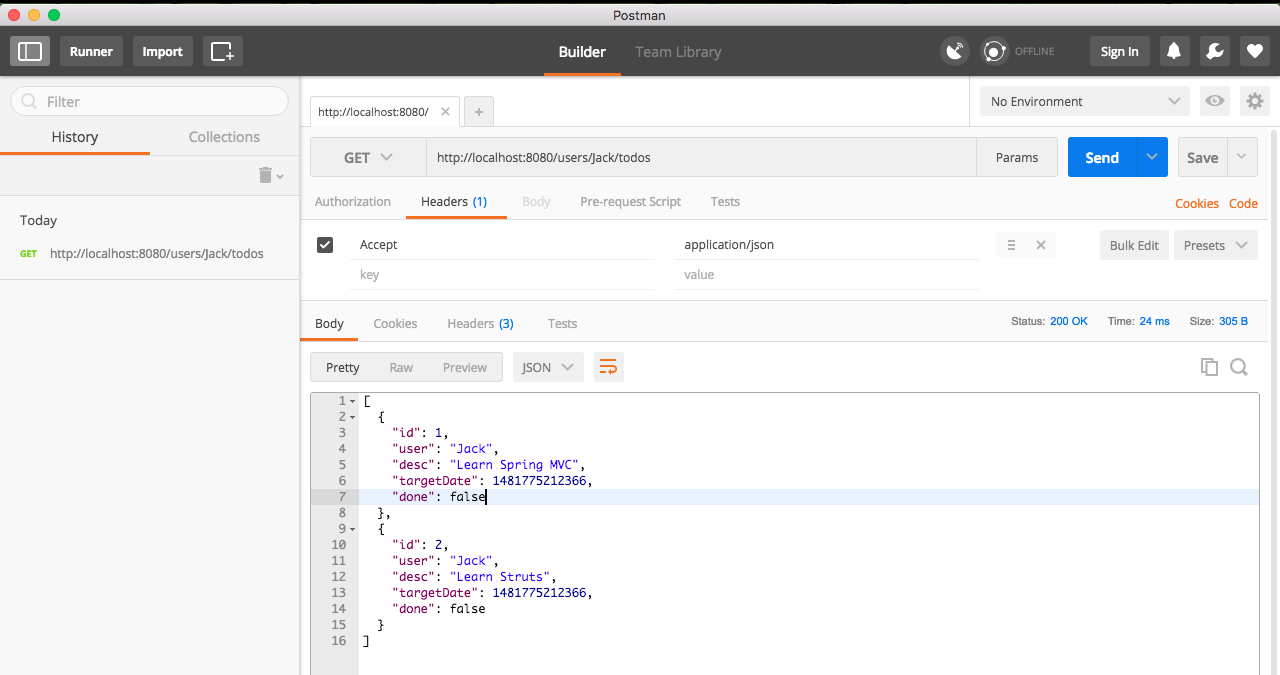
\includegraphics[scale=0.4]{img/002.png}
		\caption{Postman}
		\label{fig: 002}
	\end{center}
\end{figure}

Per creare un todo usando POST, dovremmo includere un JSON per il todo nel body della richiesta. L'interfaccia è molto intuitiva: si sceglie il tipo di richiesta sopra a sinistra, si sceglie formato raw e si avvia.

\paragraph{Unit testing}
\begin{lstlisting}[language = Java]
@Test
public void createTodo() throws Exception {
	
	Todo mockTodo = new Todo(CREATED_TODO_ID, "Jack", "Learn Spring MVC", new Date(), false);

	String todo = "{"user":"Jack","desc":"Learn Spring MVC", "done":false}";

	when(service.addTodo(anyString(), anyString(), isNull(),anyBoolean()))
		.thenReturn(mockTodo);
	
	mvc
	.perform(MockMvcRequestBuilders
		.post("/users/Jack/todos")
		.content(todo)
		.contentType(MediaType.APPLICATION_JSON)
	)
		.andExpect(status().isCreated())
		.andExpect(
			header()
				.string("location", containsString("/users/Jack/todos/"	+ CREATED_TODO_ID)));
}
\end{lstlisting}
Notiamo:
\begin{itemize}
	\item \textbf{String todo = "{"user":"Jack","desc":"Learn Spring
		MVC","done":false}"}: Prepara il contenuto da postare
	\item \textbf{when(service \\
		.addTodo(anyString(), anyString(), \\
			isNull(), anyBoolean()))
		.thenReturn(mockTodo)}: Crea un mock del servizio per ritornare un todo dummy
	\item \textbf{MockMvcRequestBuilders.post("/users/Jack/todos")
		.content(todo)
		.contentType(MediaType.APPLICATION\_JSON))}: Crea un POST riferito ad una URI specifica con il content type stabilito
	\item \textbf{andExpect(status().isCreated())}: Attende che lo status sia creato
	\item \textbf{andExpect(header().string("location",
		containsString("/users/Jack/todos/" +
			CREATED\_TODO\_ID)))}: Attende che l'hader contenga location con l'URI della risorsa creata
\end{itemize}

\paragraph{Integration testing}
\begin{lstlisting}[language = Java]
@Test
public void addTodo() throws Exception {
	
	Todo todo = new Todo(-1, "Jill", "Learn Hibernate", new Date(), false);
	
	URI location = template
		.postForLocation(createUrl("/users/Jill/todos") ,todo);
	
	assertThat(location.getPath(), containsString("/users/Jill/todos/4"));
}
\end{lstlisting}

\begin{itemize}
	\item \textbf{URI location =
		template.postForLocation(createUrl("/users/Jill/todos"),
		todo)}: postForLocation è un metodo di utilità utile nei test per creare nuove risorse. Stiamo postando il todo verso l'URI per ricevere la location dall'header
	\item \textbf{assertThat(location.getPath(), 
		containsString("/users/Jill/todos/4"))}: fa un assert sulla location contenente il path della nuova risorsa
\end{itemize}

\section{Capitolo 6: Estendere i microservizi}
\subsection{Gestione delle eccezioni}
\subsubsection{Gestione delle eccezioni di default di Spring Boot}
\paragraph{Risorsa non esistente}

Immaginiamo di chiamare una URL non esistente (http://localhost:8080/non-existing-resource), avremmo come risposta:
\begin{lstlisting}[language = ]
{
	"timestamp": 1484027734491,
	"status": 404,
	"error": "Not Found",
	"message": "No message available",
	"path": "/non-existing-resource"
}
\end{lstlisting}
Notiamo lo status 404.

\paragraph{Eccezione lanciata da una risorsa}
Creiamo una risorsa che lancia un'eccezione e inviamo una richiesta GET per capire come l'applicazione reagisca alle eccezioni a runtime.
\begin{lstlisting}[language = Java]
@GetMapping(path = "/users/dummy-service")
public Todo errorService() {
	throw new RuntimeException("Some Exception Occured");
}
\end{lstlisting}
Notiamo:
\begin{itemize}
	\item Stiamo creando un servizio GET con l'URI /users/dummy-service
	\item Il servizio lancia una RuntimeException
\end{itemize}

Se ora contattiamo http://localhost:8080/users/dummy-service la risposta sarà:
\begin{lstlisting}[language = ]
{
	"timestamp": 1484028119553,
	"status": 500,
	"error": "Internal Server Error",
	"exception": "java.lang.RuntimeException",
	"message": "Some Exception Occured",
	"path": "/users/dummy-service"
}
\end{lstlisting}

Notiamo lo status 500 e, soprattutto, il messaggio dell'eccezione.

\paragraph{Lanciare un'eccezione personalizzata}
\begin{lstlisting}[language = Java]
public class TodoNotFoundException extends RuntimeException {
	public TodoNotFoundException(String msg) {
		super(msg);
	}
}
\end{lstlisting}
Questa è un'eccezione personalizzata base.

Ora potenziamo il nostro controller in modo che lanci l'eccezione quando un todo con l'ID passato non esiste:
\begin{lstlisting}[language = Java]
@GetMapping(path = "/users/{name}/todos/{id}")
public Todo retrieveTodo(@PathVariable String name,
	@PathVariable int id) {
	Todo todo = todoService.retrieveTodo(id);
	if (todo == null) {
		throw new TodoNotFoundException("Todo Not Found");
	}
	
	return todo;
}
\end{lstlisting}
Quindi ora, nel caso il todo non venga trovato, verrà lanciata un'eccezione personalizzata.

\paragraph{Personalizzare il messaggio di errore}
\begin{lstlisting}[language = Java]
public class ExceptionResponse extends RuntimeException{
	
	private Date timestamp = new Date();
	private String message;
	private String details;

	public ExceptionResponse(String message, String details) {
		super();
		this.message = message;
		this.details = details;
	}
	
	public Date getTimestamp() {
		return timestamp;
	}

	public String getMessage() {
		return message;
	}
	
	public String getDetails() {
		return details;
	}
}
\end{lstlisting}
Così l'eccezione viene autonomamente popolata.

Quando la TodoNotFoundException viene lanciata vogliamo che venga restituita la risposta usando il bean ExceptionResponse. Possiamo creare una gestione globale delle eccezioni tramite un ControllerAdvice:
\begin{lstlisting}[language = Java]
@ControllerAdvice
@RestController
public class RestResponseEntityExceptionHandler extends ResponseEntityExceptionHandler{

	@ExceptionHandler(TodoNotFoundException.class)
	public final ResponseEntity<ExceptionResponse> todoNotFound(TodoNotFoundException ex) {
		
		ExceptionResponse exceptionResponse = new ExceptionResponse( ex.getMessage(), "Any details you would want to add");
	
	return new ResponseEntity<ExceptionResponse> (exceptionResponse, new HttpHeaders() HttpStatus.NOT_FOUND);
	}
}
\end{lstlisting}

Notiamo:
\begin{itemize}
	\item \textbf{RestResponseEntityExceptionHandler extends \\
		ResponseEntityExceptionHandler}: Estendiamo ResponseEntityExceptionHandler, che è la classe base offerta da Sring MVC per centralizzare la gestione delle eccezioni nei ControllerAdvice
	\item \textbf{@ExceptionHandler(TodoNotFoundException.class)}: Definisce che il metodo che segue gestirà tutte le eccezioni di TodoNotFoundException.class
	\item \textbf{ExceptionResponse exceptionResponse = new \\
		ExceptionResponse(ex.getMessage(), 
		"Any details you would want to add")}: Crea una nuova exception response
	\item \textbf{new ResponseEntity<ExceptionResponse>
		(exceptionResponse,new HttpHeaders(), 
		HttpStatus.NOT\_FOUND)}: Restituisce una risposta 404 resource not found
\end{itemize}

Ora quando contatteremo http://localhost:8080/users/Jack/todos/222 riceveremo come risposta:
\begin{lstlisting}[language = ]
{
	"timestamp": 1484030343311,
	"message": "Todo Not Found",
	"details": "Any details you would want to add"
}
\end{lstlisting}

Se volessimo gestire tutte le eccezioni in un modo specifico avremmo:
\begin{lstlisting}[language = Java]
@ExceptionHandler(Exception.class)
public final ResponseEntity<ExceptionResponse> todoNotFound(
	Exception ex) {
	//Customize and return the response
}
\end{lstlisting}

Ricordiamo una cosa: specifico > generale, quindi se ci sarà una gestione specifica partirà quella, altrimenti questa per tutte le altre.
\begin{table}[]
\begin{tabular}{|l|l|}
\hline
\textbf{Situazione}                                                                                                                                                    & \textbf{Response status}  \\ \hline
\begin{tabular}[c]{@{}l@{}}La request body non incontra le specifiche dell'API,\\ Non contiene dettagli sufficienti o contiene errori\\ di validazione\end{tabular}    & 400 BAD REQUEST           \\ \hline
Autenticazione o autorizzazione fallita                                                                                                                                & 401 UNAUTHORIZED          \\ \hline
\begin{tabular}[c]{@{}l@{}}L'tente non può eseguire una data operazione a\\ causa di vari fattori come una richiesta eccessiva\\ per i suoi limiti\end{tabular}        & 402 FORBIDDEN             \\ \hline
La risorsa non esiste                                                                                                                                                  & 404 NOT FOUND             \\ \hline
\begin{tabular}[c]{@{}l@{}}Operazione non supportata, per esempio, provare\\ un POST su di una risorsa dove solo GET\\ è consentito\end{tabular}                       & 405 METHOD NOT ALLOWED    \\ \hline
\begin{tabular}[c]{@{}l@{}}Errore del server. Idealmente non dovrebbe accadere.\\ L'utente non dovrebbe poter fare niente per\\ risolvere questo problema\end{tabular} & 500 INTERNAL SERVER ERROR \\ \hline
:D                                                                                                                                                                     & 418 I'M A TEAPOT          \\ \hline
\end{tabular}
\end{table}

\subsection{HATEOAS}
HATEOAS è uno degli obblighi delle applicazioni REST. 

Spiegato in parole semplice, HATEOAS impone che le API siano navigabili come se fossero una pagina web, devono avere quindi la proprietà di "discoverability", ovvero si deve poter conoscere l'insieme di azioni praticabili.

Ad esempio, questa è la risposta ricevuta visitando http://localhost:8080/todos:
\begin{lstlisting}[language = ]
{
	"_embedded" : {
		"todos" : [ {
			"user" : "Jill",
			"desc" : "Learn Hibernate",
			"done" : false,
			"_links" : {
				"self" : {
					"href" : "http://localhost:8080/todos/1"
				},
				"todo" : {
					"href" : "http://localhost:8080/todos/1"
				}
			}
		}]
	}	,
	
	"_links" : {
		"self" : {
			"href" : "http://localhost:8080/todos"
		},
		"profile" : {
			"href" : "http://localhost:8080/profile/todos"
		},
		"search" : {
			"href" : "http://localhost:8080/todos/search"
		}
	},
}
\end{lstlisting}

Se l'utente vuole fare una ricerca ha l'opzione per prendere l'URL di ricerca dalla response e inviare una richiesta ad essa. Ciò ridurrebbe il coupling tra i provider e il consumer.

\subsubsection{Inviare HATEOAS link in risposta}
Per fare un esempio su come costruirlo, potenziamo retrieveTodo (/users/{name}/todos/{id}) in modo che restituisca anche un link per recuperare tutti i todo (/users/{name}/todos):
\begin{lstlisting}[language = Java]
@GetMapping(path = "/users/{name}/todos/{id}")
public Resource<Todo> retrieveTodo(
	@PathVariable String name, 
	@PathVariable int id) {

	Todo todo = todoService.retrieveTodo(id);
	if (todo == null) {
		throw new TodoNotFoundException("Todo Not Found");
	}
	
	Resource<Todo> todoResource = new Resource<Todo>(todo);

	ControllerLinkBuilder linkTo = linkTo(methodOn(this.getClass()).retrieveTodos(name));
	
	todoResource.add(linkTo.withRel("parent"));
	
	return todoResource;
}
\end{lstlisting}
Notiamo:
\begin{itemize}
	\item \textbf{ControllerLinkBuilder linkTo = \\
		linkTo(methodOn(this.getClass()) \\
		.retrieveTodos(name))}: Vogliamo ottenere il link collegato al metodo retrieveTodos
	\item \textbf{linkTo.withRel("parent")}: La relazione con la corrente relazione è quella di "parent"
\end{itemize}

Ora la risposta a hettp://localhost:8080/users/Jac/todos/1 sarà:
\begin{lstlisting}[language = ]
{
	"id": 1,
	"user": "Jack",
	"desc": "Learn Spring MVC",
	"targetDate": 1484038262110,
	"done": false,
	
	"_links": {
		"parent": {
			"href": "http://localhost:8080/users/Jack/todos"
		}
	}
}
\end{lstlisting}

\subsection{Validazione}
Ogni buon servizio validerà sempre i dati prima di processarli (SQL injection, anyone?).

Le Bean Validation API offrono un numero di annotazioni che possono essere usate per validare i bean. 

\subsubsection{Abilitare la validazione su di un metodo di un controller}
\begin{lstlisting}[language = Java]
@RequestMapping(method = RequestMethod.POST, path = "/users/{name}/todos")
ResponseEntity<?> add(@PathVariable String name
	@Valid @RequestBody Todo todo) {
	
	...
	
}
\end{lstlisting}
L'annotazione @Valid è usata per segnare un parametro per la validazione. Ogni validazione è definita nel bean Todo è eseguita prima che ilmetodo add sia eseguito.

\subsubsection{Definire la validazione del bean}
Aggiungiamo le validazioni sui campi del Todo bean:
\begin{lstlisting}[language = Java]
public class Todo {	

	private int id;

	@NotNull
	private String user;
	
	@Size(min = 9, message = "Enter at least 10 Characters.")
	private String desc;
\end{lstlisting}

Notiamo:
\begin{itemize}
	\item \textbf{@NotNull}: Controlla che il campo non sia vuoto
	\item \textbf{@Size(min = 9, \\
		message = "Enter at least 10 Characters.")}: Controlla che il campo abbia almeno 10 caratteri
\end{itemize}

\subsubsection{Annotazioni per la validazione}
Ci sono svariate annotazioni, eccone alcune:
\begin{itemize}
	\item \textbf{@AssertFalse, @AssertTrue}: Per i booleani. Controlla il loro valore
	\item \textbf{@Assert}: controlla che il valore sia vero
	\item \textbf{@Future}: La data deve essere nel futuro
	\item \textbf{@Past}: Controlla che la data sia nel passato
	\item \textbf{@Max}: annota un numero che deve essere minore o uguale al valore specificato
	\item \textbf{@Min}: annota un numero che deve essere maggiore o uguale al valore specificato
	\item \textbf{@NotNull}: Il valore non può essere null
	\item \textbf{@Pattern}: La stringa annotata deve rispettare la regex collegata
	\item \textbf{@Size}: L'elemento deve rientrare in una lunghezza massima
\end{itemize}

\subsubsection{Unit Testing}
\begin{lstlisting}[language = Java]
@Test
public void createTodo_withValidationError() throws Exception {
	
	Todo mockTodo = new Todo(CREATED_TODO_ID, "Jack", "Learn Spring MVC", new Date(), false);

	String todo = "{"user":"Jack","desc":"Learn","done":false}";

	when( service.addTodo(anyString(), anyString(), isNull(), anyBoolean()))
		.thenReturn(mockTodo);
	
	MvcResult result = mvc.perform(MockMvcRequestBuilders
		.post("/users/Jack/todos")
			.content(todo)
			.contentType(MediaType.APPLICATION_JSON))
		.andExpect(status().is4xxClientError())
		.andReturn();
}
\end{lstlisting}
Notiamo:
\begin{itemize}
	\item \textbf{"desc":"Learn"}: Stiamo usando una descrizione con lunghezza 5 quando abbiamo detto che deve essere almeno 10 caratteri
	\item \textbf{.andExpect(status().is4xxClientError())}: Controlla per gli errori di validazione
\end{itemize}

\subsection{Documentare un servizio REST}
Un "contratto" è ciò che definisce i dettagli del servizio:
\begin{itemize}
	\item Come posso chiamarlo? Qual è l'URI?
	\item Quale dovrebbe essere il formato della richiesta?
	\item Che tipo di risposta dovrei attendere?
\end{itemize}
Ci sono svariate opzioni per definire un contratto per un servizio RESTful. Il più popolare è Swagger. 

\subsubsection{Creare una specifica di Swagger}
Springfox Swagger può essere utilizzato per generare la documentazione dal codice. In più c'è uno strumento chiamato Swagger UI che, integrato con l'applicazione, offre documentazione leggibile.

Semplicemente bisogna inserire nel pom.xml:
\begin{lstlisting}[language = XML]
<dependency>
	<groupId>io.springfox</groupId>
	<artifactId>springfox-swagger2</artifactId>
	<version>2.4.0</version>
</dependency>

<dependency>
	<groupId>io.springfox</groupId>
	<artifactId>springfox-swagger-ui</artifactId>
	<version>2.4.0</version>
</dependency>
\end{lstlisting}
Lo step successivo è quello di abilitare e generare la documentazione swagger:
\begin{lstlisting}[language = Java]
@Configuration
@EnableSwagger2
public class SwaggerConfig {

	@Bean
	public Docket api() {
		return new Docket(DocumentationType.SWAGGER_2)
			.select()
			.apis(RequestHandlerSelectors.any())
			.paths(PathSelectors.any()).build();
	}
}
\end{lstlisting}

Notiamo:
\begin{itemize}
	\item \textbf{@Configuration}: Crea un file di coniguazione Spring
	\item \textbf{@EnableSwagger2}: Abilita swagger
	\item \textbf{Docket}: Un semplice builder per configurare la generazione della documentazione swagger usando Swagger Spring MVC Framework
	\item \textbf{new Docket(DocumentationType.SWAGGER\_2)}: Configura Swagger 2 come versione
	\item \textbf{.apis(RequestHandlerSelectors.any())\\
		.paths(PathSelectors.any())}: Include tutte le API e i path nella documentazione
\end{itemize}

Quindi, quando interrogheremo http://localhost:8080/v2/api-docs, otteremo:
\begin{figure}[h!]
	\begin{center}
		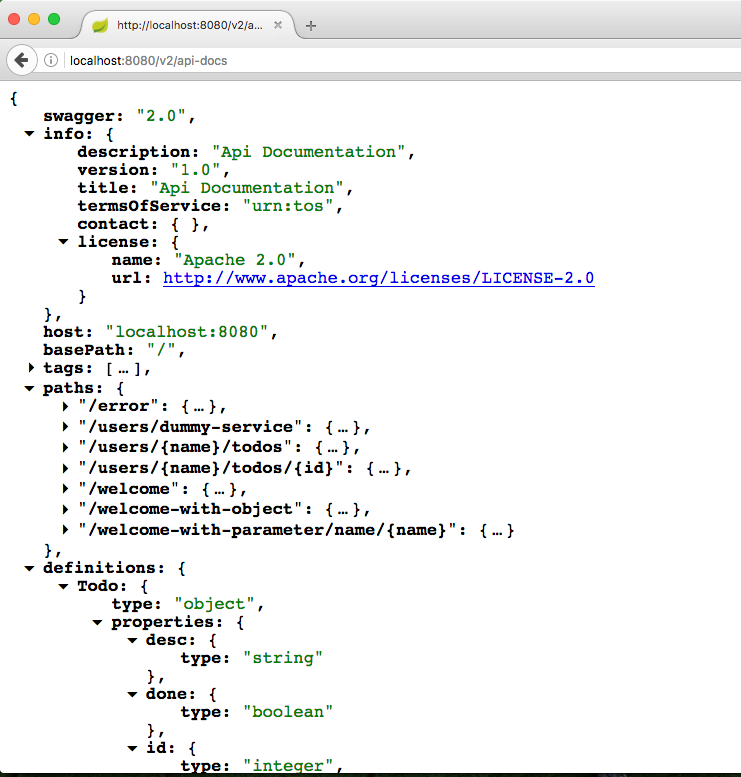
\includegraphics[scale=0.6]{img/003.png}
		\caption{Documentazione Swagger}
		\label{fig: 003}
	\end{center}
\end{figure}
Ad esempio, questa è la documentazione per recupeare il servizio todos:
\begin{lstlisting}[language = ]
"/users/{name}/todos": {
	"get": {
		"tags": [
			"todo-controller"
		],
		
		"summary": "retrieveTodos",
		"operationId": "retrieveTodosUsingGET",

		"consumes": [
			"application/json"
		],
		
		"produces": [
			"*/*"
		],
		
		"parameters": [{
			"name": "name",
			"in": "path",
			"description": "name",
			"required": true,
			"type": "string"
		}],
		
	"responses": {
		"200": {
			"description": "OK",
			"schema": {
				"type": "array",
				items": {
					"$ref": "#/definitions/Todo"
				}
			}
		},
	
		"401": {
			"description": "Unauthorized"
		},
		
		"403": {
			"description": "Forbidden"
		},
		
		"404": {
			"description": "Not Found"
		}
	}
}
\end{lstlisting}

Il servizio definisce una richiesta e una risposta al servizio. Sono anche definite le differenti risposte ai vari status.

Questa invece la definizione del bean Todo:
\begin{lstlisting}[language = ]
"Resource<Todo>": {
	"type": "object",
	"properties": {
		"desc": {
			"type": "string"
		},
	
		"done": {
			"type": "boolean"
		},
		
		"id": {
			"type": "integer",
			"format": "int32"
		},
	
		"links": {
			"type": "array",
			"items": {
				"$ref": "#/definitions/Link"
			}
		},
	
		"targetDate": {
			"type": "string",
			"format": "date-time"
		},
		
		"user": {
			"type": "string"
		}
	}
}
\end{lstlisting}

\paragraph{Swagger UI}
Swagger UI è un modo comodissimo per avere una vista molto intuitiva dei vari servizi e degli endpoint. Offre la possibilità di visualizzare la documentazione (Swagger JSON) in maniera alternativa.

\begin{figure}[h!]
	\begin{center}
		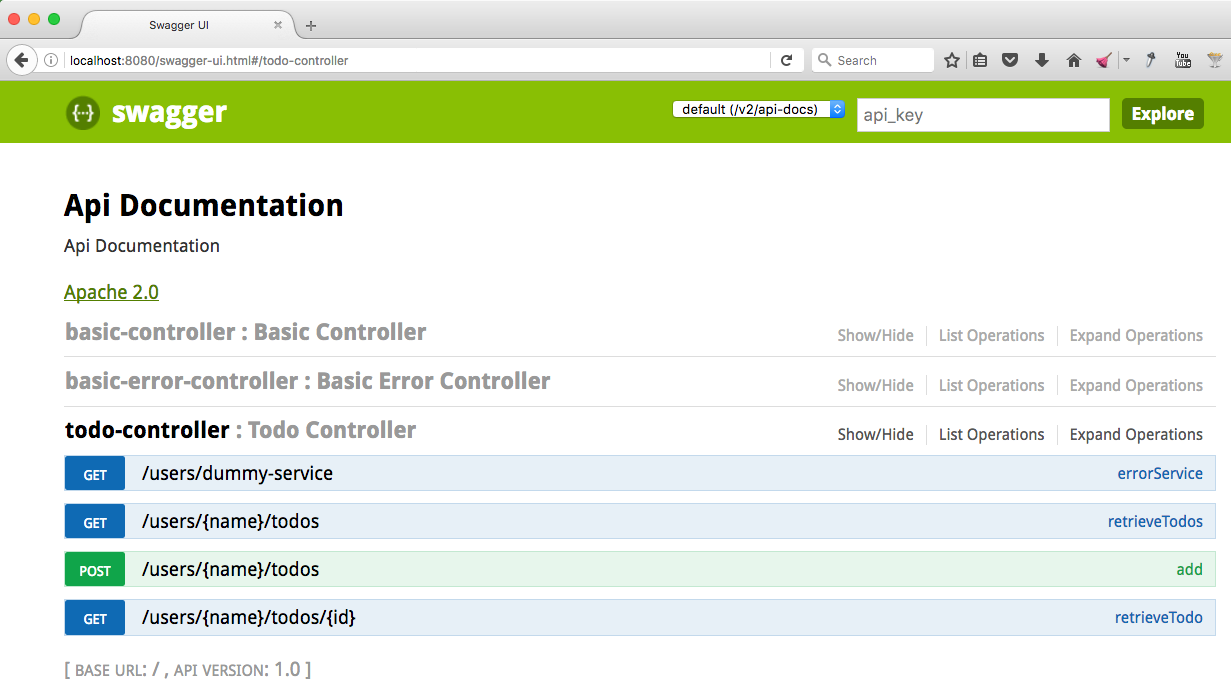
\includegraphics[scale=0.4]{img/004.png}
		\caption{Visualizzazione della documentazione}
		\label{fig: 004}
	\end{center}
\end{figure}

\begin{figure}[h!]
	\begin{center}
		
\includegraphics[scale=0.6]{img/005.png}
		\caption{Esempio di elemento POST}
		\label{fig: 005}
	\end{center}
\end{figure}

Notiamo:
\begin{itemize}
	\item \textbf{Parameters} mostra tutti i parametri importanti inclusi quelli del request body
	\item \textbf{Parameters type} mostra tutta la struttura del body della richiesta
	\item \textbf{Response messages} mostra differenti status HTTP ritornati dal servizio
\end{itemize}

\paragraph{Personalizzare la documentazione con le annotazioni}
Swagger offre delle annotazioni che vengono aggiunte ai servisi RESTful per personalizzare la documentazione:
\begin{lstlisting}[language = Java]
@ApiOperation(
	value = "Retrieve all todos for a user by passing in his name",
	notes = "A list of matching todos is returned. Current pagination is not supported." response = Todo.class, responseContainer = "List" produces = "application/json")
@GetMapping("/users/{name}/todos")
public List<Todo> retrieveTodos(@PathVariable String name) {
	return todoService.retrieveTodos(name);
}
\end{lstlisting}

Notiamo:
\begin{itemize}
	\item \textbf{@ApiOperation(value = "Retrieve all todos\\
		for a user by passing in his name")}: Produce la documentazione come un riassunto del servizio
	\item \textbf{notes = "A list of matching todos is returned.\\ 
		Current pagination is not supported."}: Prodotto nella documentazione come descrizione del servizio
	\item \textbf{produces = "application/json”}: Personalizza la sezione produces della documentazione
\end{itemize}

\begin{lstlisting}[language = ]
# Documentazione prima

"get": {
	"tags": [
	"todo-controller"
	],
	"summary": "retrieveTodos",
	"operationId": "retrieveTodosUsingGET",
	"consumes": [
		"application/json"
	],
	"produces": [
		"*/*"
	]
	
	...
}

# Documentazione dopo
get": {
	"tags": [
		"todo-controller"
	],
	"summary": "Retrieve all todos for a user by passing in his name",
	"description": "A list of matching todos is returned. Current pagination is not supported.",
	"operationId": "retrieveTodosUsingGET", 
	"consumes": [
		"application/json"
	],
	"produces": [
		"application/json",
	"*/*"
	]
	
	...
}
\end{lstlisting}

\subsubsection{Lista di annotazioni Swagger}
\begin{itemize}
	\item \textbf{@Api}: Segna la classe come risorsa per Swagger
	\item \textbf{@ApiModel}: Offre informazioni addizionali sul modello
	\item \textbf{@ApiModelProperty}: Agiunge e manipola i dati delle proprietà di un model
	\item \textbf{@ApiOperation}: Descrive un'operazione o un metodo HTTP rispetto allo specifico path
	\item \textbf{@ApiParam}: Agginge dei metadati addizionali per i parametri dell'operazione
	\item \textbf{@ApiResponse}: Decrive un esempio di risposta di un operazione
	\item \textbf{@ApiResponses}: Un wrapper per consentire una lista di più oggetti @ApiResponse
	\item \textbf{@Authorization}: Dichiara uno schema di autorizzazione da utilizzare su di una risorsa o un'operazione
	\item \textbf{@AuthorizationScope}: Descrive uno scope di autorizzazione OAuth 2
	\item \textbf{@ResponseHeader}: Rappresenta l'header che può essere fornito come parte della risposta
\end{itemize}

In più Swagger offre una serie di annotazioni che possono essere usate per personalizzare le informazioni di alto livello riguardanti un gruppo di servizi (contatti, licenze e altre informazioni). Tra questi:
\begin{itemize}
	\item \textbf{@SwaggerDefinition}: proprietà a livello di definizione che può essere aggiunta per generare una definizione di Swagger
	\item \textbf{@Info}: Metadati generali per una definizione di Swagger
	\item \textbf{@Contact}: Proprietà per descrivere una persona che deve essere contattata per una definizione di Swagger
	\item \textbf{@License}: Proprietà per descrivere una licenza per una proprietà di Swagger
\end{itemize}

\subsection{Mettere in sicurezza un servizio REST con Spring Security}
Da inserire tramite file pom.xml:
\begin{lstlisting}[language = XML]
<dependency>
	<groupId>org.springframework.boot</groupId>
	<artifactId>spring-boot-starter-security</artifactId>
</dependency>
\end{lstlisting}

\subsubsection{Autenticazione base}
Spring security blocca tutti i servizi in maniera automatica. La risposta base ad ogni richiesta è:
\begin{lstlisting}[language = ]
{
	"timestamp": 1484120815039,
	"status": 401,
	"error": "Unauthorized",
	"message": "Full authentication is required to access this
	resource",
	"path": "/users/Jack/todos"
}
\end{lstlisting}

Spring richiede quindi uno user ID e una password. Non avendole ancora impostate, Spring security imposta automaticamente uno user la cui password è nel log di sistema.

Con postman possiamo inviare una richiesta con i dati di autenticazione.

Possiamo anche configurare lo userID e la password in application.properties. Spring security offre anche la possibilità di autenticarsi tramite LDAP o JDBC.

\paragraph{Integration testing}
\begin{lstlisting}[language = Java]
private TestRestTemplate template = new TestRestTemplate();
HttpHeaders headers = createHeaders("user-name", "user-password");

HttpHeaders createHeaders(String username, String password) {
	return new HttpHeaders() {{
		String auth = username + ":" + password;
		byte[] encodedAuth = Base64.getEncoder().encode(auth
			.getBytes(Charset.forName("US-ASCII")));
		String authHeader = "Basic " + new String(encodedAuth);
		set("Authorization", authHeader);
		}
	};
}

@Test
public void retrieveTodos() throws Exception {
	String expected = "["
		+ "{id:1,user:Jack,desc:\"Learn Spring MVC\",done:false}" + ","
		+ "{id:2,user:Jack,desc:\"Learn Struts\",done:false}" + "]";
	
	ResponseEntity<String> response = template.exchange(
		createUrl("/users/Jack/todos"), HttpMethod.GET, new HttpEntity<String>(null, headers), String.class);

	JSONAssert.assertEquals(expected, response.getBody(), false);
}
\end{lstlisting}

Notiamo:
\begin{itemize}
	\item \textbf{createHeaders("user-name", "user-password")}: crea un header di autenticazione in base64\footnote{Base64 è un sistema di codifica che consente la traduzione di dati binari in stringhe di testo ASCII, rappresentando i dati sulla base di 64 caratteri ASCII diversi. Viene usato principalmente come codifica di dati binari nelle e-mail, per convertire i dati nel formato ASCII.}
	\item \textbf{ResponseEntity<String> response =	
		template.exchange(createUrl("/users/Jack/todos"),
		HttpMethod.GET,new HttpEntity<String>(null, headers),
		String.class)}: HttpEntity offre l'header che abbiamo creato prima al template REST
\end{itemize}	

\paragraph{Unit testing}
\begin{lstlisting}[language = Java]
@RunWith(SpringRunner.class)
@WebMvcTest(value = TodoController.class, secure = false)
public class TodoControllerTest {
\end{lstlisting}

Semplicemente mettere "secure = false" disabilità spring secure per il test.

\subsubsection{Autenticazione Oauth 2}
Permette ad applicazioni terze di ottenere informazioni ristrette dell'utente tramite il servizio.

Consideriamo un esempio. Vogliamo esporre le nostre API su internet. In questo scambio OAuth 2 sono importanti queste parti:
\begin{itemize}
	\item \textbf{Resource owner}: È l'utente dell'applicazione di terze parti che vuole usare le nostre API. Decide quante informazioni rendere disponibili alle API
	\item \textbf{Resource server}: Offre le API, le risorse che vogliamo mettere al sicuro
	\item \textbf{Client}: L'applicazione dei terze parti che vuole usare le API
	\item \textbf{Authorization server}: È il server che offre il servizio OAuth
\end{itemize}

\subsubsection{Flow di alto livello}
Il flow è:
\begin{enumerate}
	\item L'applicazione richiede che l'utente autorizzi l'accesso alle API
	\item L'utente offre l'accesso, l'applicazione riceve il consenso
	\item L'applicazione offre all'utente il consenso all'autorizzazione e le sue credenziali all'authorization server
	\item Se l'autenticazione è positiva, l'authorization server risponde con un token d'accesso
	\item L'applicazione chiama le API (il resource server) che offre il token d'accesso per l'autenticazione
	\item Se il token è valido, le risorse ritornano i dettagli della risorsa
\end{enumerate}

\subsubsection{Implementare l'autenticazione OAuth 2}
Solitamente il server di autorizzazione sarebbe differente rispetto a quello dove l'API è esposta.

Questo snippet mostra come abilitare l'applicazione ad agire come server di autenticazione:
\begin{lstlisting}[language = Java]
@EnableResourceServer
@EnableAuthorizationServer
@SpringBootApplication
public class Application {
\end{lstlisting}
Notiamo:
\begin{itemize}
	\item \textbf{@EnableResourceServer}: Abilita un filtro di Spring Security che autentica le richieste tramite un token OAuth 2
	\item \textbf{@EnableAuthorizationServer}: Abilita un EuthorizationEndpoint e un TokenEndpoint nel contesto dell'applicazione corrente, che sarà il DispatcherServlet
\end{itemize}

Ora possiamo configurare i dettagli dell'accesso in application.properties:
\begin{lstlisting}[language = ]
security.user.name=user-name
security.user.password=user-password
security.oauth2.client.clientId: clientId
security.oauth2.client.clientSecret: clientSecret
security.oauth2.client.authorized-grant-types:
authorization_code,refresh_token,password
security.oauth2.client.scope: openid
\end{lstlisting}

Notiamo:
\begin{itemize}
	\item \textbf{security.user.name and\\
		security.user.password}: sono i dettagli per il resource owner
	\item \textbf{security.oauth2.client.clientId and \\
		security.oauth2.client.clientSecret}: sono i dettagli per l'autenticazione del client che è definito nelle applicazioni di terze parti
\end{itemize}

\paragraph{Eseguire una richiesta OAuth}
Abbiamo bisogno di due passaggi:
\begin{enumerate}
	\item Ottenere un token di accesso
	\item Eseguire una richiesta usando il token di accesso
\end{enumerate}

\paragraph{Ottenere un token di accesso}
Per ottenere il token chiamiamo il server passando i dettagli di autenticazione. Inviando in POST i dettagli della richiesta otteniamo come risposta qualcosa di simile a ciò:
\begin{lstlisting}[language = ]
{
	"access_token": "a633dd55-102f-4f53-bcbd-a857df54b821",
	"token_type": "bearer",
	"refresh_token": "d68d89ec-0a13-4224-a29b-e9056768c7f0",
	"expires_in": 43199,
	"scope": "openid"
}
\end{lstlisting}

Notiamo:
\begin{itemize}
	\item \textbf{access\_token}: Le applicazioni client possono usare il token di accesos per autenticare altre chiamate API. Solitamente il token scade in poco
	\item \textbf{refresh\_token}: Le applicazioni client possono passare una nuova richiesta al server di autenticazione con il refresh\_token per ottenere un nuovo access\_token.
\end{itemize}

\paragraph{Integration test}
\begin{lstlisting}[language = Java]
@Test
public void retrieveTodos() throws Exception {
	String expected = "["
		+ "{id:1,user:Jack,desc:\"Learn Spring MVC\",done:false}" + ","
		+"{id:2,user:Jack,desc:\"Learn Struts\",done:false}" + "]";
	
	String uri = "/users/Jack/todos";
	ResourceOwnerPasswordResourceDetails resource =
		new ResourceOwnerPasswordResourceDetails();

	resource.setUsername("user-name");
	resource.setPassword("user-password");
	resource.setAccessTokenUri(createUrl("/oauth/token"));
	resource.setClientId("clientId");
	resource.setClientSecret("clientSecret");
	resource.setGrantType("password");

	OAuth2RestTemplate oauthTemplate = new OAuth2RestTemplate(resource,new DefaultOAuth2ClientContext());
	
	ResponseEntity<String> response = oauthTemplate.getForEntity(createUrl(uri), String.class);
	
	JSONAssert.assertEquals(expected, response.getBody(), false);
}
\end{lstlisting}

Notiamo:
\begin{itemize}
	\item \textbf{ResourceOwnerPasswordResourceDetails resource = \\
	new ResourceOwnerPasswordResourceDetails()}: Prepariamo ResourceOwnerPasswordResourceDetails con le credenziali dell'utente e del client
	\item \textbf{resource.setAccessTokenUri(\\
		createUrl("/oauth/token"))}: Configura l'URL del server di autenticazione	
	\item \textbf{OAuth2RestTemplate oauthTemplate = \\
		new OAuth2RestTemplate(resource, \\
		new DefaultOAuth2ClientContext())}: OAuth2RestTemplate è un'estensione del RestTemplate, che supporta il protocollo OAuth 2
\end{itemize}

\subsection{Internazionalizzazione}
È il processo di sviluppare un'applicazione e i servizi in modo che siano personalizzati per lingue differenti e culture nel mondo. È anche chiamata localizzazione. Spring Boot ha un servizio di internazionalizzazione OOTB.

Abbiamo prima di tutto bisogno di un LocaleResolver:
\begin{lstlisting}[language = Java]
@Bean
public LocaleResolver localeResolver() {
	SessionLocaleResolver sessionLocaleResolver = new SessionLocaleResolver();
	sessionLocaleResolver.setDefaultLocale(Locale.US);
	
	return sessionLocaleResolver;
}

@Bean
public ResourceBundleMessageSource messageSource() {
	ResourceBundleMessageSource messageSource = new ResourceBundleMessageSource();
	messageSource.setBasenames("messages");
	messageSource.setUseCodeAsDefaultMessage(true);
	
	return messageSource;
}
\end{lstlisting}
Notiamo:
\begin{itemize}
	\item \textbf{sessionLocaleResolver.setDefaultLocale(Locale.US)}: Settiamo il default locale con Locale.US
	\item \textbf{messageSource.setBasenames("messages")}: Settiamo il nome della fonte di base dei messaggi come messages. Le varie fonti vengono prese dai file message\_[sigla locale].properties.
	\item \textbf{messageSource.setUseCodeAsDefaultMessage(true)}: Se un messagio non è trovato allora il codice è ritornato come messaggi di default
\end{itemize}

I vari file semplicemente conterranno i campi con la loro definizione, ad esempio:
\begin{lstlisting}[language = ]
# message_en.properties

welcome.message=Welcome in English

# message_fr.properties

welcome.message=Welcome in French
\end{lstlisting}

Per poi invocarlo in maniera semplice con il locale specificato nell'header "Accept-Language":
\begin{lstlisting}[language = Java]
@GetMapping("/welcome-internationalized")
public String msg(@RequestHeader(value = "Accept-Language", required = false) Locale locale) {

	return messageSource.getMessage("welcome.message", null, locale);
}
\end{lstlisting}

Notiamo:
\begin{itemize}
	\item \textbf{@RequestHeader(value = "Accept-Language", \\
		required = false) Locale locale}: Il locale è confiurato tramite la request header Accept-Language. Non è essenziale. Se un locale non è specificato viene usato quello di default.
	\item \textbf{messageSource.getMessage("welcome.message", \\
		null, locale)}: messageSource è autowired nel controller. 
\end{itemize}

\subsection{Caching}
La cache ha un ruolo essenziale nelle performance e nalla scalabilità delle applicazioni. Spring offre un'astrazione basata sulle annotazioni.

\subsubsection{Spring-boot-starter-cache}
Come sempre basta una piccola agigunta a pom.xml:
\begin{lstlisting}[language = XML]
<dependency>
	<groupId>org.springframework.boot</groupId>
	<artifactId>spring-boot-starter-cache</artifactId>
</dependency>
\end{lstlisting}

\subsubsection{Abilitare il caching}
\begin{lstlisting}[language = Java]
@EnableCaching
@SpringBootApplication
public class Application {
\end{lstlisting}

Yup, basta @EnableCaching.

\subsubsection{Caching data}
Ora che abbiamo abilitato il caching possiamo aggiungere l'annotazione @Cachable ai metodi di cui vogliamo mettere in cache i dati. 
\begin{lstlisting}[language = Java]
@Cacheable("todos")
public List<Todo> retrieveTodos(String user) {
\end{lstlisting}

I Todo per uno specifico utente sono messi nella cache. Sono anche ammesse condizioni:
\begin{lstlisting}[language = Java]
@Cacheable(cacheNames="todos", condition=#user.length < 10)
public List<Todo> retrieveTodos(String user) {
\end{lstlisting}

\paragraph{Annotazioni per il caching}
\begin{itemize}
	\item \textbf{@CachePut}: Aggiunge esplicitamente i dati alla cache
	\item \textbf{@CacheEvict}: Rimuove i dati dalla cache
	\item \textbf{@Caching}: Permette più annotazioni innestate sullo stesso metodo
\end{itemize}

\section{Capitolo 7: Feature avanzate di Spring Boot}
\subsection{Configurazioni esternalizzate}
Spring boot offre un modo flessibile e standardizzato per gestire i file di configurazione esterni.

\subsubsection{Personalizzare i framework attraverso application.properties}
\paragraph{Logging}
Alcune cose che possono essere personalizzate:
\begin{itemize}
	\item Il path del file di configurazione per il logging
	\item Il path dell'output
	\item Il livello di logging
\end{itemize}

\begin{lstlisting}[language = ]
#  Posizione del file di logging
	logging.config=
# Nome del log.
	logging.file=
# Configurare il livello di logging.
# Esempio `logging.level.org.springframework=TRACE`
	logging.level.*=
\end{lstlisting}

\paragraph{Configurazione del server embedded}
Il server embedded di Spring è una delle caratteristiche più importanti. Tra le cose che si possono configurare:
\begin{itemize}
	\item Porte
	\item Supporto SSL e configurazione
	\item Configurazione dell'access log
\end{itemize}

\begin{lstlisting}[language = ]
# Path dell'errore per i controller.
	server.error.path=/error
# Server HTTP port.
	server.port=8080
# Abilitare il supporto SSL.
	server.ssl.enabled=
# Percorso del key store per l'SSL
	server.ssl.key-store=
# Key Store Password
	server.ssl.key-store-password=
# Key Store Provider	
	server.ssl.key-store-provider=
# Key Store Type
	server.ssl.key-store-type=
# Abilitazione del log degli accessi a Tomcat?
	server.tomcat.accesslog.enabled=false
# Numero massimo di connessioni accettate
	server.tomcat.max-connections=
\end{lstlisting}

\paragraph{Spring MVC}
Spring MVC può essere configurato tramite application.properties. Ad esempio:
\begin{lstlisting}[language =]
# Formato della data `dd/MM/yyyy`.
	spring.mvc.date-format=
# Locale da usare.
	spring.mvc.locale=
# Definire come il locale dovrebbe essere impostato.
	spring.mvc.locale-resolver=accept-header
# Bisognerebbe lanciare una "NoHandlerFoundException"
# nel caso l'handler non venisse trovato?
	spring.mvc.throw-exception-if-no-handler-found=false
# Prefisso per Spring MVC. Usato dal view resolver.
	spring.mvc.view.prefix=
# Suffisso per Spring MVC. Usato dal view resolver.
	spring.mvc.view.suffix=
\end{lstlisting}

\paragraph{Spring Starter Security}

\begin{lstlisting}[language = ]
# Impostare vero per la sicurezza base
	security.basic.enabled=true
# Lista di path da mettere in sicurezza divisi da virgole
	security.basic.path=/**
# Lista di path da NON mettere in sicurezza divisi da virgole
	security.ignored=
# Nome dello user di base configurato da SPring Security
	security.user.name=user
# Password dell'utente base definito da Spring
	security.user.password=
# Ruolo dello user
	security.user.role=USER
\end{lstlisting}

\paragraph{Basi di dati}

\begin{lstlisting}[language = ]
# Nome completo del driver JDBC
	spring.datasource.driver-class-name=
# Popolare il database usando 'data.sql'.
	spring.datasource.initialize=true
# Posizione JNDI della fonte dati.
	spring.datasource.jndi-name=
# Nome della fonte dati.
	spring.datasource.name=testdb
# Password di login del database.
	spring.datasource.password=
# Puntatore allo script di creazione DB.
	spring.datasource.schema=
# Db User per eseguire gli script
	spring.datasource.schema-username=
# Db password per eseguire gli scripts
	spring.datasource.schema-password=
# Url JDBC del database.
	spring.datasource.url=
# JPA - Inizializza lo schema all'avvio.
	spring.jpa.generate-ddl=false
# Use Hibernate's newer IdentifierGenerator for AUTO, TABLE and SEQUENCE.
	spring.jpa.hibernate.use-new-id-generator-mappings=
# Enable logging of SQL statements.
	spring.jpa.show-sql=false
\end{lstlisting}

\paragraph{Altre configurazioni}
Ad esempio:
\begin{itemize}
	\item Profili
	\item Convertitori di messaggi HTTP (Jackson/JSON)
	\item Gestione delle transazioni
	\item Internazionalizzazione
\end{itemize}

\begin{lstlisting}[language = ]
# Comma-separated list (or list if using YAML) of active profiles.spring.profiles.active=
# HTTP message conversion. jackson or gson
	spring.http.converters.preferred-json-mapper=jackson
# JACKSON Date format string. Example `yyyy-MM-dd HH:mm:ss`.
	spring.jackson.date-format=
# Default transaction timeout in seconds.
	spring.transaction.default-timeout=
# Perform the rollback on commit failures.
	spring.transaction.rollback-on-commit-failure=
# Internationalisation : Comma-separated list of basenames
	spring.messages.basename=messages
# Cache expiration for resource bundles, in sec. -1 will cache for ever
	spring.messages.cache-seconds=-1
\end{lstlisting}

\subsubsection{Proprietà personalizzate in application.properties}
Consideriamo un esempio: vogliamo avere la possibilità di interagire con un servizio esterno. Vogliamo quindi poter esternalizzare la configurazione dell'URL di questo servizio.

Vogliamo quindi configurarlo in application.properties così:
\begin{lstlisting}[language = ]
somedataservice.url=http://abc.service.com/something
\end{lstlisting}

Vogliamo usare il valore di somedataservice.url nel nostro service. 

\begin{lstlisting}[language = Java]
@Component
public class SomeDataService {
	
	@Value("${somedataservice.url}")
	private String url;

	public String retrieveSomeData() {
		// Logic using the url and getting the data
	
		return "data from service";
	}
}
\end{lstlisting}

Notiamo:
\begin{itemize}
	\item \textbf{@Component public class SomeDataService}: Il bean è gestito da Spring
	\item \textbf{@Value("\${somedataservice.url}")}: il calore di somedataservice.url sarà autowired all'url.
\end{itemize}

\paragraph{Configuration manager type-safe}
Nel caso si volessero impostare più elementi tramite properties ci sono due possibilità:
\begin{itemize}
	\item Apporre l'annotazione @Value su tutti i campi
	\item Usare l'annotazione @ConfigurazionProperties("nome file di proprietà")
\end{itemize}

In maniera molto semplice il secondo definisce tutte le associazioni e poi vengono collegate all'interno del file.

\begin{lstlisting}[language = Java]
@Component
@ConfigurationProperties("application")
public class ApplicationConfiguration {
	
	private boolean enableSwitchForService1;
	private String service1Url;
	private int service1Timeout;

	public boolean isEnableSwitchForService1() {
		return enableSwitchForService1;
	}
	
	public void setEnableSwitchForService1
		(boolean enableSwitchForService1) {
		this.enableSwitchForService1 =
			enableSwitchForService1;
	}
	
	public String getService1Url() {
		return service1Url;
	}

	public void setService1Url(String service1Url) {
		this.service1Url = service1Url;
	}

	public int getService1Timeout() {
		return service1Timeout;
	}

	public void setService1Timeout(int service1Timeout) {
		this.service1Timeout = service1Timeout;
	}
}
\end{lstlisting}

Notiamo:
\begin{itemize}
	\item \textbf{@ConfigurationProperties("application")}: Seleziona il file di proprietà da utilizzare. 
	\item Così configuriamo più bean in una volta sola
	\item Getter e Setter sono richiesti
\end{itemize}

In maniera molto semplice i valori sono salvati in application.properties:
\begin{lstlisting}[language = ]
application.enableSwitchForService1=true
application.service1Url=http://abc-dev.service.com/
	somethingelse
application.service1Timeout=250
\end{lstlisting}

\subsubsection{Profili}
Per ora abbiamo visto come esternalizzare i file di configurazione, ma se volessimo differenti valori per differenti ambienti?

I profili sono ciò che arrivano in aiuto. In application.properties:
\begin{lstlisting}[language =]
spring.profiles.active=dev
\end{lstlisting}

Ora che abbiamo selezionato il profilo possiamo usare dei file di configurazione specializzati per profilo usando la notazione \textbf{application-{profile-name}.properties}.

\paragraph{Configurazione dei bean basata sul profilo}
Tutte le classi che sono annotate con @Component (o le sue versioni più specifiche) o @Configuration possono essere annotate anche con \textbf{@Profile(profilo)}.

Ad esempio:
\begin{lstlisting}[language = Java]
// Dev
@Profile("dev")
@Configuration
public class DevSpecificConfiguration {
	
	@Bean
	public String cache() {
		return "Dev Cache Configuration";
	}
}

// Production

@Profile("prod")
@Configuration
public class ProdSpecificConfiguration {
	
	@Bean
	public String cache() {
		return "Production Cache Configuration - Distributed Cache";
	}
}
\end{lstlisting}


\subsubsection{Altre opzioni per i valori di configurazione}
Spring offre svariate possibilità per configurare le proprietà delle applicazioni. Ad esempio:
\begin{itemize}
	\item Argomenti via linea di comando
	\item Creare delle proprietà di sistema col nome SPRING\_APPLICATION\_JSON e includere una configurazione JSON
	\item ServetConfig init
	\item ServletContext init
	\item Proprietà di Java (System.getProperties())
	\item Variabili di sistema
	\item Proprietà specifiche per il profilo
	\item Proprietà fuori dal .jar
	\item Proprietà all'interno del .jar
\end{itemize}

\subsubsection{Configurazione YAML}
YAML sta per "YAML Ain't Markup Language". È un formato leggibile ed è usato spesso per i file di configurazione. Per fare un esempio:
\begin{lstlisting}[language = ]
spring:
	profiles:
		active: prod
security:
	basic:
		enabled: false
	user:
		name=user-name
		password=user-password
	oauth2:
		client:
			clientId: clientId
			clientSecret: clientSecret
			authorized-grant-types: authorization_code,refresh_token,password
			scope: openid

application:
	enableSwitchForService1: true
	service1Url: http://abc-dev.service.com/somethingelse
	service1Timeout: 250
\end{lstlisting}

YAML permette anche la definizione di vari profili, sempre in maniera molto semplice:
\begin{lstlisting}[language =]
application:
	service1Url: http://service.default.com
---
spring:
	profiles: dev
	application:
		service1Url: http://service.dev.com
---
spring:
	profiles: prod
	application:
		service1Url: http://service.prod.com
\end{lstlisting}


\section{Capitolo 8: Spring Data}

\section{Capitolo 9: Spring Cloud}

\section{Capitolo 10: Spring Cloud Data Flow}

\section{Capitolo 11: Programmazione Reactive}

\section{Capitolo 12: Spring Best Practices}

\chapter{Introducing Spring Boot - Udemy}
\href{https://www.udemy.com/course/spring-boot-getting-started/}{Spring boot - getting started}.

\section{Spring initializr}
\href{https://start.spring.io/}{Spring Initializr}, no, non è un typo.

Questo sito permette di creare velocemente un template che seleziona direttamente tutte le dipendenze.

In project Metadata abbiamo group, ovvero il nome del package di default, e artifact che sarà il nome del progetto, il tipo di wrapper (jar/war) e la versione del compilatore.

Nelle dipendenze possiamo dire quali dipendenze vogliamo.
\begin{figure}[h!]
	\begin{center}
		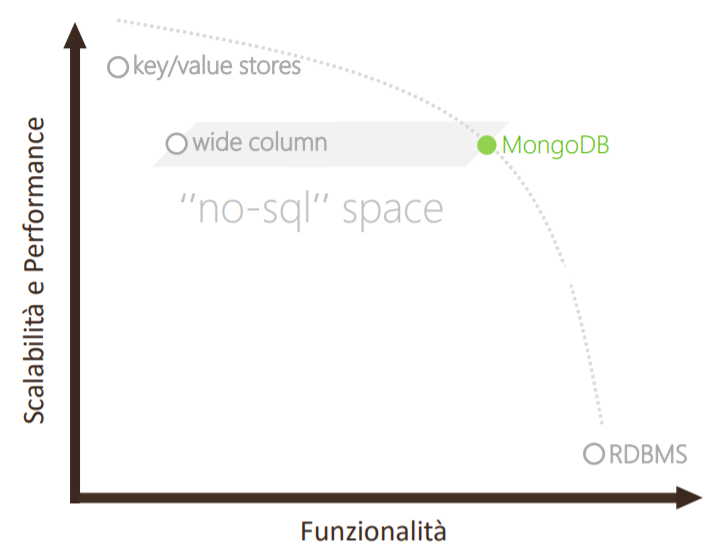
\includegraphics[scale=0.6]{img/001.png}
		\caption{Spring Initializr}
		\label{fig: 001}
	\end{center}
\end{figure}
Ad esempio con questa configurazione otteniamo i file all'interno della cartella \href{Codici/SpringInitializr}{SpringInitializr}.

Anche Spring CLI ci permette di eseguire la stessa funzione, per avere una lista delle possibilità scrivere "spring init -list" in una console. Per fare un esempio scriviamo "spring init -d=web my-app", dove -d sta per le dipendenze e my-app sarà il nome dell'applicazione.

Spring Initializr è integrato anche in molte IDE.

\section{Java Build Tools}
Un build tool è un sistema di scripting per automatizzare alcuni compiti. Tre tra i più importanti sono:
\begin{itemize}
	\item \href{https://ant.apache.org/}{Ant}, ormai poco usato
	\item \href{https://maven.apache.org/}{Maven}. Offre la gestione delle dipendenze, è basato sui plugin e crea un file di configurazione XML
	\item \href{https://gradle.org/}{Gradle}. È basato su groovy.
\end{itemize}
Non c'è molta differenza tra Maven e Gradle.

\subsection{Maven build}
Aprendo il file \href{Codici/SpringInitializr/Maven/pom.xml}{pom.xml} possiamo vedere la dichiarazione della versione di spring boot usata.
\begin{lstlisting}[language = XML]
<parent>
	<groupId>org.springframework.boot</groupId>
	<artifactId>spring-boot-starter-parent</artifactId>
	<version>2.2.2.RELEASE</version>
	<relativePath/> <!-- lookup parent from repository -->
</parent>
\end{lstlisting}

Nella prima parte troviamo anche i nostri metadati:
\begin{lstlisting}[language = XML]
<groupId>com.example</groupId>
<artifactId>demo</artifactId>
<version>0.0.1-SNAPSHOT</version>
<name>demo</name>
<description>Demo project for Spring Boot</description>
\end{lstlisting}

Vedremo anche la sezione delle dipendenze. Ad esempio:
\begin{lstlisting}[language = XML]
<dependencies>
	<dependency>
		<groupId>org.springframework.boot</groupId>
		<artifactId>spring-boot-starter-data-jpa
			</artifactId>
	</dependency>
	<dependency>
		<groupId>org.springframework.boot</groupId>
		<artifactId>spring-boot-starter-web</artifactId>
	</dependency>
</dependencies>
\end{lstlisting}
Notare che non abbiamo dovuto segnare alcuna versione per le dipendenze.

La versione di Java:
\begin{lstlisting}[language = XML]
<properties>
	<java.version>1.8</java.version>
</properties>
\end{lstlisting}

Successivamente c'è la sezione per la build, in modo da definire il tipo di file wrapper.
\begin{lstlisting}[language = XML]
<build>
	<plugins>
		<plugin>
			<groupId>org.springframework.boot
				</groupId>
			<artifactId>spring-boot-maven-plugin
				</artifactId>
		</plugin>
	</plugins>
</build>
\end{lstlisting}

Infine, per eseguire il progetto Spring boot possiamo scrivere nella console "mvn spring-boot:run"

\subsubsection{Starter POM}
È molto facile crearne uno, \href{https://docs.spring.io/spring-boot/docs/current-SNAPSHOT/reference/htmlsingle/#using-boot-starter}{qua} la documentazione e \href{https://www.baeldung.com/spring-boot-starters}{qua} una spiegazione più discorsiva.

Ad esempio possiamo vedere tra le dipendenze "spring-boot-starter-web", per importare un ambiente fullstack completo di tomcat e spring web MVC.

\subsection{Gradle build}
Il file di build è \href{Codici/SpringInitializr/Gradle/build.gradle}{build.gradle}.

Differentemente da Maven, non abbiamo un superparent da cui importare le impostazioni di default.

All'inizio viene fissata la versione si SpringBoot e dei vari plugin:
\begin{lstlisting}[language = XML]
plugins {
	id 'org.springframework.boot' version '2.2.2.RELEASE'
	id 'io.spring.dependency-management' version '1.0.8.RELEASE'
	id 'java'
}
\end{lstlisting}

Le dipendenze possono essere importate velocemente:
\begin{lstlisting}[language = XML]
dependencies {
	implementation 'org.springframework.boot: spring-boot-starter-data-jpa'
	implementation 'org.springframework.boot: spring-boot-starter-web'
	developmentOnly 'org.springframework.boot: spring-boot-devtools'
	testImplementation('org.springframework.boot: spring-boot-starter-test') {
		exclude group: 'org.junit.vintage', 
		module: 'junit-vintage-engine'
	}
}
\end{lstlisting}

\section{DevTools e live reload}
DevTools non viene incluso all'interno del jar finale. Dev tools offre alcuni sturmenti utili durante la fase dello sviluppo, ad esempio il mantenimento della cache (spring.thymeleaf.cache) per velocizzare l'app, ha sistemi di restart automatico ogni volta che viene compilata una classe (spring loaded e JRebel). C'è anche un live reload, ovvero un estensione browser che aggiorna la pagina ad ogni cambiamento lato server.

\section{Spring boot}
Iniziamo scrivendo un controller in un file groovy. Il file HelloWorld.groovy si occuperà semplicemente di mostrare la stringa "Hello, World!" sul browser.
\href{Codici/HelloWorld.groovy}{Qua il codice}. 

\section{Executable JAR}
I JAR sono archivi che contengono le classi compilate con tutte le loro dipendenze. Sono cloud friendly, nel senso che possono essere direttamente caricate online sul server.

Java non offre nessun metodo diretto per caricare file jar innestati. Spring boot offre anche questa funzione.

Maven: "mvn package" \\
Gradle: "gradle boot"

Per creare il jar scrivere "spring jar [nome jar] [file da includere]"

\chapter{Spring Core}
\begin{center}
	\textbf{Learn Spring Framework 4 and Spring Boot}
\end{center} 
\href{https://www.udemy.com/course/spring-core}{Spring Core - Learn Spring Framework 4 and Spring Boot}
\href{https://springframework.guru/spring-framework-annotations/}{Sito dell'istruttore}

Le caratteristiche principali di spring sono:
\begin{itemize}
	\item Beans: Spring usa POJO (plain Old Java Objects) o "Spring beans"
	\item Dependecy injection (DI): 
	\item Inversion of Control (IoC)
\end{itemize}

\section{Hello World}
\href{Codici/HelloWorld2}{Codice}

\begin{lstlisting}[language = Java]
@Component
public class HelloWorld {
    public void sayHello(){
        System.out.println("Hello world!");
    }
}
\end{lstlisting}
Possiamo notare che la nostra classe HelloWorld è registrata come component. Questo vuol dire che Spring interpreterà la classe come un bean. La cosa risulta utile all'interno dell'applicazione:

\begin{lstlisting}[language = Java]
@SpringBootApplication
public class HelloworldApplication {
    public static void main(String[] args) {
        ApplicationContext ctx = SpringApplication
        	.run(HelloworldApplication.class, args);

        HelloWorld helloWorld = (HelloWorld) ctx.getBean("helloWorld");
        helloWorld.sayHello();  
    }
}
\end{lstlisting}
Analizziamo un attimo questo codice:
\begin{itemize}
	\item @SpringBootApplication: Permette all'applicazione di attivare tre funzioni automaticamente:
	\begin{itemize}
		\item @EnableAutoConfiguration: Cerca di configurare automaticamente Spring in base alle dipendenze inserite
		\item @ComponentScan: cerca automaticamente i @Component nel package dell'applicazione
		\item @Configuration: Permette di registrare beans extra nel contesto o importare classi di configurazione addizionali
	\end{itemize}
	\item ApplicationContext: serve per ricevere le configurazioni dell'applicazione
	\item ctx.getBean: Spring cerca tra i vari bean (component) uno che abbia quel nome e lo passa come oggetto
	\item (HelloWorld): il casting serve perchè altrimenti l'application context passerebbe un oggetto
\end{itemize}

\section{Dependecy Injection}
È una della componenti principali di Spring. L'applicazione si occupa di collegare automaticamente gli oggetti ai loro beans. Questo approccio, ovvero partire dall'oggetto dipendente per risalire, è il concetto dell'IoC. Il lato positivo dell'IoC è il poter usare diversi bean a runtime e riduce la coesione del codice, in modo da poter rendere più indipendenti le classi.

Ci sono più tipi di dependecy injection:
\begin{itemize}
	\item \textbf{Basata sui costruttori}. Preferito per le classi che non possono essere istanziate senza le loro dipendenze
	\item \textbf{Basata sui setter}. Preferito nelle applicazioni di Spring, più flessibile dei costruttori.
	\item \textbf{Basata sulle interfacce}. È considerata la best practice. È allineata con i principi della programmazione orientata agli oggetti. Permette flessibilità nella composizione delle classi.
\end{itemize}

Per capire meglio come usare autowired andare a pagina \pageref{par: Autowired}.

\subsection{Profili}
\href{Codici/Controllers}{Codice}.

Abbiamo creato un controller che si occupa di generare un'istanza di HelloWorldService e restituire il suo saluto.
\begin{lstlisting}[language = Java]
@Controller
public class GreetingController {

    private HelloWorldService helloWorldService;

    @Autowired
    public void setHelloWorldService (HelloWorldService helloWorldService) {
        this.helloWorldService = helloWorldService;
    }

    public String sayHello(){
        String greeting = helloWorldService.getGreeting();

        System.out.println(greeting);

        return greeting;
    }
}
\end{lstlisting}
Possiamo riconoscere la sua natura dall'annotazione Controller. QUando viene creato un GreetingController viene attivato Autowired su setHelloWorldService e verrà creato uno dei componenti disponibili.

\begin{lstlisting}[language = Java]
// Interfaccia
public interface HelloWorldService {
    public String getGreeting();
}

//_______________________________
//HelloWorldServiceEnglishImpl

@Component
@Profile("english")
public class HelloWorldServiceEnglishImpl implements HelloWorldService {

    @Override
    public String getGreeting() {
        return "Hello world";
    }
}

//_______________________________
//HelloWorldServiceSpanishImpl

@Component
@Profile("spanish")
public class HelloWorldServiceSpanishImpl implements HelloWorldService{

    @Override
    public String getGreeting() {
        return "Hola Mundo";
    }
}

\end{lstlisting}
Come fa il controller a distinguere tra le varie versioni e sapere quale implementare? Notare che nelle due implementazioni abbiamo l'annotazione Profile con un tag. Nel file .properties abbiamo creato appositamente una stringa "spring.profiles.active=english" per segnalare al controller che il profilo che vogliamo in questo momento è quello inglese.

\subsection{Default profiles}
Annotare un bean con "@Profile("default")" viene automaticamente riconosciuto da Spring come un profilo speciale, ovvero quello di base se non è presente alcuna annotazione nel file di proprietà.

Per poter usare una classe sia come profilo di defult che come classe normale si possono usare più profili, basta scrivere all'interno delle annotazioni tutti i nomi separati da virgole e racchiunderli tra graffe. \\ E.g. @Profile({"it", "default"})


\section{Spring Java Configuration}
\subsection{Component scan}
Come detto precedentemente, Component scan funziona cercando i vari bean all'interno del suo package. Se volessimo dire di cercare anche altri bean all'interno di altri package dovremmo scrivere tra le annotazioni sopra la classe "@ComponentScan("[nome package]")".

\textbf{Attenzione!}: quando si chiede un bean al contesto il nome deve iniziare con la minuscola, anche se la classe ha un nome che inizia con una maiuscola.

\subsection{Spring Java Configuration classes}
\begin{lstlisting}[language = Java]
@Configuration
public class HelloConfig {

    @Bean
    @Profile("default, english")
    public HelloWorldService helloWorldServiceEnglish(){
        return new HelloWorldServiceEnglishImpl();
    }
    
    @Bean
    @Profile("spanish")
    public HelloWorldService helloWorldServiceSpanish(){
        return new HelloWorldServiceSpanishImpl();
    }
}

\end{lstlisting}

Possiamo svolgere la stessa funzione creando un file di configurazione per istanziare tutti i bean. Le annotazioni da usare sono Configuration, Bean e Profile come visto precedentemente.

Perchè usare un file di configurazione? È usato di solito con librerie di terze parti perchè non avendo accesso al codice sorgente ci si deve adattare.
\subsection{Factory beans}
\href{Codici/Beans}{Codice}.

Si usa solitamente quando ci si deve collegare ad un database.
\begin{lstlisting}[language = Java]
public class HelloWorldFactory {

    public HelloWorldService 
    	createHelloWorldService(String language){
        HelloWorldService service = null;

        switch (language){
            case "en":
                service = new HelloWorldServiceEnglishImpl();
                break;
            case "es":
                service =  new HelloWorldServiceSpanishImpl();
                break;
            case "fr":
                service = new HelloWorldServiceFrenchImpl();
                break;
            case "de":
                service =  new HelloWorldServiceGermanImpl();
                break;
            case "pl":
                service = new HelloWorldServicePolish();
                break;
            case "ru":
                service = new HelloWorldServiceRussianImpl();
                break;
            default: 
            	new HelloWorldServiceEnglishImpl();
        }

        return service;
    }
 }

\end{lstlisting}
Abbiamo creato una factory che in base alla configurazione scelta inizializza un bean differente.  Questo viene effettuato passando attraverso il file di configurazione:
\begin{lstlisting}[language = Java]
@Configuration
public class HelloConfig {

    @Bean
    public HelloWorldFactory helloWorldFactory(){
        return new HelloWorldFactory();
    }

    @Bean
    @Profile("english")
    public HelloWorldService HelloWorldServiceEnglish(HelloWorldFactory factory){
        return factory.createHelloWorldService("en");
    }
}
\end{lstlisting}
Come possiamo vedere ora Il file di configurazione crea una Factory che viene passata all'istanziazione dell'HelloWorldService.
\subsection{Opzioni avanzate per Autowire}
\begin{lstlisting}[language = Java]
@Configuration
public class HelloConfig {

    @Bean
    public HelloWorldFactory helloWorldFactory(){
        return new HelloWorldFactory();
    }

    @Bean
    @Profile("english")
    @Primary
    public HelloWorldService helloWorldServiceEnglish(HelloWorldFactory factory){
        return factory.createHelloWorldService("en");
    }
    
    @Bean
    @Profile("spanish")
    public HelloWorldService helloWorldServiceSpanish(HelloWorldFactory factory){
        return factory.createHelloWorldService("es");
    }
}
\end{lstlisting}
L'annotazione Primary segnala a Spring che se non viene chiesto niente allora il bean da preferire è quello.

Si può anche usare l'injection in maniere più elaborate, ad esempio:
\begin{lstlisting}[language = Java]
@Configuration
public class HelloConfig {

    @Bean
    public HelloWorldFactory helloWorldFactory(){
        return new HelloWorldFactory();
    }

    @Bean
    @Profile("english")
    @Primary
    public HelloWorldService helloWorldServiceEnglish(HelloWorldFactory factory){
        return factory.createHelloWorldService("en");
    }
    
    @Bean
    @Profile("spanish")
    public HelloWorldService helloWorldServiceSpanish(HelloWorldFactory factory){
        return factory.createHelloWorldService("es");
    }
    

    @Bean("french")
    public HelloWorldService helloWorldServiceFrench(HelloWorldFactory factory){
        return factory.createHelloWorldService("fr");
    }
    
    @Bean
    public HelloWorldService helloWorldServiceDeutsche(HelloWorldFactory factory){
        return factory.createHelloWorldService("de");
    }
}

// _____________________________________________

//_____________________________________________

private HelloWorldService helloWorldService;

    private HelloWorldService helloWorldServiceGerman;

    private HelloWorldService helloWorldServiceFrench;


	// Wired tramite Primary
    @Autowired
    public void setHelloWorldService (HelloWorldService helloWorldService) {
        
        this.helloWorldService = helloWorldService;
    }

	// Wired tramite identifier (nome del bean)
    @Autowired
    @Qualifier("helloWorldServiceGerman") 
    public void setHelloWorldServiceGerman (HelloWorldService helloWorldServiceGerman) {
        this.helloWorldServiceGerman = 
        	helloWorldServiceGerman;
    }

	// Wired tramite nome del bean
	// (equivalente a Qualifier)
    @Autowired
    @Qualifier("french")
    public void setHelloWorldServiceFrench (HelloWorldService helloWorldServiceFrench) {
        
        this.helloWorldServiceFrench = helloWorldServiceFrench;
    }
\end{lstlisting}

\section{Configurazione tramite XML}
IntelliJ aiuta già dando tra le opzioni anche la creazione di un file apposito per spring. Qua inseriremo prima di tutto la tag per la component scan all'interno della quale indicheremo il/i nostro/i package per la ricerca dei bean.

All'interno del main inseriremo il tag @ImportResource("classpath:[locazione sotto la cartella resources per il file di configurazione]")

Cose fighe: se abbiamo una factory per i bean non dichiariamo direttamente il bean con la sua classe ma in questo modo:
\begin{lstlisting}[language = XML]
<bean id="helloWorldServiceFactory" 
	class="com.example.springtest.demo
	.service.HelloWorldServiceFactory" />

<bean id="italian" factory-bean="helloWorldServiceFactory" factory-method="helloWorldServiceCreate">
	<constructor-arg value="it" />
</bean>
\end{lstlisting}

Un vantaggio dei file di configurazione è che se ne possono creare di più da integrare in parti separate del progetto tramite @ImportResource. In questo modo si possono personalizzare i valori di default e le configurazioni in base alla sezione.


\chapter*{Siti utili}
\href{http://docs.spring.io/spring-boot/docs/current/reference/htmlsingle}{Documentazione Spring boot} \\
\href{http://docs.spring.io/spring-boot/docs/current/api/}{Documentazione Spring API} \\
\href{http://spring.io/projects}{Piattafroma Spring IO} \\
\href{http://spring.io/guides}{Guide} \\
\href{https://docs.spring.io/spring-boot/docs/current/reference/html/spring-boot-cli.html}{Spring CLI} \\
\href{Codici/SpringInitializr}{SpringInitializr} \\
\href{https://www.webjars.org/}{Per portare velocemente risorse nel progetto}. Quando si aggiunge una dipendenza bisogna inserirla in pom.xml e poi fare mvn install. \\
\href{https://projectlombok.org/}{Lombok}. \\
\href{https://sdkman.io/}{Per gestire versioni parallele di più ambienti di sviluppo} \\
\href{https://www.postman.com/}{Postman}. \\
\href{https://swagger.io/tools/swagger-ui/}{Swagger UI} \\

\end{document}
